\documentclass{article}

%change margins
\usepackage[a4paper, left=2cm, right=2cm, top=2.5cm, bottom=2.5cm]{geometry}
%placement accuracy
\usepackage{float}
% Needed for custom title page
\usepackage{titling} 
\usepackage{array}
%for figures
\usepackage{graphicx}
\usepackage{subcaption}

%for coding highlighting
\usepackage{listings}
\usepackage{xcolor}

\lstdefinestyle{cppstyle}{
    language=C++,
    basicstyle=\ttfamily\footnotesize,
    keywordstyle=\color{blue},
    commentstyle=\color{gray},
    stringstyle=\color{teal},
    backgroundcolor=\color{white},
    frame=single,
    breaklines=true,
    breakatwhitespace=false,
    tabsize=4,
    showstringspaces=false,
    captionpos=b
}
%3 commands beloew needed for greek text
\usepackage{fontspec} 
\usepackage[greek,english]{babel}
\setmainfont{Times New Roman}

\title{\Huge Analysis of Branch Prediction Techniques \\[1em] using the PIN Tool}
\author{
  \textbf{Χαράλαμπος Παπαδόπουλος\\ 03120199} \\[3cm]
  {Προηγμένα Θέματα Αρχιτεκτονικής Υπολογιστών\\ 1η Άσκηση} \\
}
\date{Απρίλιος 2025}


\begin{document}

\begin{titlepage}
    \centering
    \vspace{3cm}

    
\includegraphics[width=4cm]{figures/emp.png}\\
    \vspace{1.5cm}
    {\fontsize{24pt}{20pt}\selectfont{Εθνικό Μετσόβιο Πολυτεχνείο}}\\[0.3cm]
    {\fontsize{16pt}{18pt}\selectfont Σχολή Ηλεκτρολόγων Μηχανικών \& Μηχανικών Υπολογιστών}\\[0.3cm]
    {\fontsize{16pt}{18pt}\selectfont Αρχιτεκτονική Υπολογιστών}\\[2cm]

    {\Huge\bfseries \thetitle \par}
    \vspace{2cm}
    {\Large \theauthor \par}
    \vfill

    {\fontsize{15pt}{18pt}Απρίλιος 2025}
\end{titlepage}


\newpage

\section{Εισαγωγή}

Στα πλαίσια της παρούσας άσκησης θα χρησιμοποιήσουμε το εργαλείο PIN για να μελετήσουμε την επίδραση διαφορετικών συστημάτων πρόβλεψης εντολών άλματος, καθώς και την αξιολόγησή τους με δεδομένο το διαθέσιμο χώρο πάνω στο τσιπ.

Στη ροή εκτέλεσης ενός προγράμματος, οι εντολές διακλάδωσης (branches) παίζουν κρίσιμο ρόλο, καθώς καθορίζουν την πορεία που θα ακολουθήσει η εκτέλεση βάσει συνθηκών και δομών ελέγχου (όπως if, for, while, κ.ά.). Οι διακλαδώσεις μπορεί να είναι υποθετικές (conditional), όπου η λήψη της απόφασης εξαρτάται από μια συνθήκη, ή ανεπιφύλακτες (unconditional), όπου η μετάβαση είναι δεδομένη.

Η πρόβλεψη διακλαδώσεων (branch prediction) είναι μία τεχνική που εφαρμόζεται σε σύγχρονους επεξεργαστές για να μειώσει την καθυστέρηση που προκαλείται από την αβεβαιότητα της εκτέλεσης τέτοιων εντολών. Οι σύγχρονοι επεξεργαστές βασίζονται σε σωληνώσεις (pipelines) και εκτέλεση πολλαπλών εντολών παράλληλα (superscalar execution), καθιστώντας τη σωστή πρόβλεψη των διακλαδώσεων κρίσιμη για τη διατήρηση της απόδοσης.

Η αποδοτικότητα ενός μηχανισμού πρόβλεψης επηρεάζει άμεσα την ταχύτητα και την ενεργειακή κατανάλωση ενός συστήματος. Ένας λανθασμένος προγνωστικός μηχανισμός μπορεί να οδηγήσει σε καθυστερήσεις, καθώς απαιτείται εκκαθάριση και ανανέωση του pipeline. Για τον λόγο αυτό, η επιλογή και αξιολόγηση της κατάλληλης στρατηγικής πρόβλεψης, ανάλογα με τον διαθέσιμο χώρο και την πολυπλοκότητα του υλικού, αποτελεί σημαντικό αντικείμενο μελέτης στην αρχιτεκτονική υπολογιστών.

\section{Ανάλυση εντολών άλματος}
Αρχικά, συλλέγουμε δεδομένα σχετικά με τα benchmarks που θα χρησιμοποιήσουμε (τόσο για τα train όσο και τα ref) χρησιμοποιώντας το pintool cslab\_branch\_stats.so. Λαμβάνουμε, λοιπόν τα εξής αποτελέσματα:

\begin{table}[h!]
    \centering

    \renewcommand{\arraystretch}{1.3}
    \begin{tabular}{|c|c|c|c|c|c|c|}
    \hline
    Benchmark & 
    \begin{tabular}[c]{@{}c@{}}Total\\[2pt]Branches\end{tabular} & 
    \begin{tabular}[c]{@{}c@{}}Conditional\\[2pt]Taken\end{tabular} & 
    \begin{tabular}[c]{@{}c@{}}Conditional\\[2pt]Not Taken\end{tabular} & 
    \begin{tabular}[c]{@{}c@{}}Unconditional\\[2pt]Branches\end{tabular} & 
    \begin{tabular}[c]{@{}c@{}}Calls\end{tabular} & 
    \begin{tabular}[c]{@{}c@{}}Returns\end{tabular} \\
    \hline
    401.bzip2 &  48731240680 & 14828890244 & 29233486500 & 4503343406 & 82760267 & 82760263 \\
    \hline
    403.gcc & 754261098 & 269641225 & 304818852 & 66609945 & 56595540 & 56595536 \\
    \hline
    410.bwaves & 31873093532 & 21133244425 & 8406203291 & 1791546316 & 271049752 & 271049748 \\
    \hline
    416.gamess &  14348669381 &  6258963398 & 6983826386 & 863109166 & 121385219 & 121385212 \\
    \hline
    429.mcf &  3862679407 & 1332802908 & 2377832566 & 97772747 & 27135595 & 27135591 \\
    \hline
    433.milc &  2240722314 & 1242012269 & 541178208 & 21600368 & 217965738 & 217965731 \\
    \hline
    435.gromacs &  18177458459 & 5651211656 & 11410526337 & 778103616 & 168808427 & 168808423 \\
    \hline
    436.cactusADM & 170600508 & 142370779 & 19042164 & 1719499 & 3734035 & 3734031 \\   
    \hline
    437.leslie3d &  17218327107 & 16400961590 & 810904801 & 4541911 & 959406 & 959399 \\
    \hline
    450.soplex &  1261449374 & 640242394 & 484809667 & 46077417 & 45159950 & 45159946 \\    
    \hline
    456.hmmer &  13914144105 & 8669664400 & 4743905013 & 94489468 & 203042614 & 203042610 \\
    \hline
    459.GemsFDTD &  3408454302 & 2895485194 & 348903461 & 50019703 & 57022974 & 57022970 \\
    \hline
    464.h264ref &  48076004067 & 24275875054 & 8491727313 & 3326070462 & 5991165621 & 5991165617 \\
    \hline
    470.lbm &  1356406164 & 176492622 & 922282496 & 252368694 & 2631178 & 2631174 \\
    \hline
    471.omnetpp &  50858988954 & 11220928577 & 21007505135 & 4549937533 & 7040308988 & 7040308721 \\
    \hline
    483.xalancbmk &  54702087725 & 8947195710 & 19089680931 & 5016363416 & 10824423836 & 10824423832 \\
    \hline
    \end{tabular}
    \caption{Branch Prediction Statistics for Train Benchmarks}
\end{table}
\begin{table}[H]
    \centering
    \renewcommand{\arraystretch}{1.3}
    \begin{tabular}{|c|c|c|c|c|c|c|}
    \hline
    Benchmark & 
    \begin{tabular}[c]{@{}c@{}}Total\\[2pt]Branches\end{tabular} & 
    \begin{tabular}[c]{@{}c@{}}Conditional\\[2pt]Taken\end{tabular} & 
    \begin{tabular}[c]{@{}c@{}}Conditional\\[2pt]Not Taken\end{tabular} & 
    \begin{tabular}[c]{@{}c@{}}Unconditional\\[2pt]Branches\end{tabular} & 
    \begin{tabular}[c]{@{}c@{}}Calls\end{tabular} & 
    \begin{tabular}[c]{@{}c@{}}Returns\end{tabular} \\
    \hline
    401.bzip2 & 45686521905 & 15926493292 & 22623211331 & 4456192564 & 1340312361 & 1340312357 \\
    \hline
    403.gcc & 33841317469 & 12296277104 & 13569715817 & 3134043792 & 2420640380 & 2420640376 \\
    \hline
    410.bwaves &  128568449445 & 88592484629 & 34014693916 & 3853748332 & 1053761286 & 1053761282 \\
    \hline
    416.gamess &  73894102026 & 34756617371 & 32132851363 & 5481923933 & 761354687 & 761354672 \\
    \hline
    429.mcf &  67874046952 & 25764447757 & 39087004417 & 2224162736 & 399216023 & 399216019 \\
    \hline
    433.milc &  67919982540 & 36675874082 & 16584640014 & 1322820263 & 6668324094 & 6668324087 \\
    \hline
    435.gromacs &  84256714798 & 26179759996 & 52980568742 & 3595806252 & 750289906 & 750289902 \\
    \hline
    436.cactusADM &  4368886354 & 4156985961 & 165208684 & 8975841 & 18857936 & 18857932 \\
    \hline
    437.leslie3d &  119714175105 & 114398465011 & 5298773071 & 14378054 & 1279488 & 1279481 \\
    \hline
    450.soplex &  57636398865 & 31511622629 & 20460639260 & 1923982890 & 1870077045 & 1870077041 \\
    \hline
    456.hmmer &  42165181169 & 27398563731 & 14228668166 & 221630014 & 158159631 & 158159627 \\
    \hline
    459.GemsFDTD &  47114377011 & 33969941316 & 7764020378 & 2457796415 & 1461309453 & 1461309449 \\
    \hline
    464.h264ref &  48076004019 & 24275874976 & 8491727354 & 3326070449 & 5991165622 & 5991165618 \\
    \hline
    470.lbm &  15278518783 & 527480913 & 11071877357 & 3673870653 & 2644932 & 2644928 \\
    \hline
    471.omnetpp &  137784824709 & 29163496937 & 63903123884 & 11932487679 & 16392858237 & 16392857972 \\
    \hline
    483.xalancbmk & 287764730034 & 75393414336 & 162510582834 & 8390230048 & 20735251410 & 20735251406 \\
    \hline

\end{tabular}
\caption{Branch Prediction Statistics for Ref Benchmarks}
\end{table}

\section{Ν-bit predictors}
Σε αυτό το ερώτημα εξετάζουμε την ανάλυση κάποιων branch predictors. Οι N-bit predictors χρησιμοποιούν περισσότερα από ένα bit για να παρακολουθήσουν την ιστορία των αποφάσεων των branch. Αντί να χρησιμοποιούν μόνο ένα bit για να καταγράψουν αν ένα branch εκτελείται ή όχι, χρησιμοποιούν έναν μετρητή που αυξάνεται ή μειώνεται με βάση τις προηγούμενες αποφάσεις. Αυτή η μέθοδος βοηθάει στην καλύτερη πρόβλεψη, καθώς καταγράφει πιο πολύπλοκες συμπεριφορές των branch.

Για παράδειγμα, ένας 2-bit predictor χρησιμοποιεί έναν μετρητή που μπορεί να έχει 4 καταστάσεις, με τις οποίες μπορεί να προβλέψει με μεγαλύτερη ακρίβεια τη συμπεριφορά ενός branch, καθώς χρειάζονται δύο συνεχόμενα λάθη για να αλλάξει η πρόβλεψη. Η χρήση περισσότερων bit (όπως 3-bit ή 4-bit) βελτιώνει ακόμη περισσότερο την ακρίβεια, αλλά απαιτεί περισσότερη μνήμη και υπολογιστική ισχύ.

\subsection{}
 Διατηρώντας σταθερό τον αριθμό των BHT entries και ίσο με 16Κ, προσομοιώνουμε τους n-bit
predictors, για Ν = 1, 2, 3, 4. Τα n-bits υλοποιούν ένα saturating up-down counter (cslab\_branch.cpp) όπως είδαμε στις διαλέξεις.
Τροποιούμε κατάλληλα τον βοηθητικό κώδικα προσθέτοντας τον εξής κώδικα
\begin{lstlisting}[style=cppstyle]
   for (int i=1; i <= 4; i++) {
       NbitPredictor *nbitPred = new NbitPredictor(14, i);
       branch_predictors.push_back(nbitPred);
   }
\end{lstlisting}
Οι παράμετροι που δίνουμε στο object \texttt{NbitPredictor} είναι:
\begin{itemize}
    \item \texttt{index\_bits = 14}~: Ορίζει το πλήθος των bits που χρησιμοποιούνται για την κατασκευή του πίνακα προβλέψεων. Δηλαδή, το μέγεθος του πίνακα θα είναι $2^{14}$ καταχωρήσεις.
    \item \texttt{cntr\_bits}~: Ορίζει το πλήθος των bits κάθε μετρητή στον πίνακα. Όσο περισσότερα bits, τόσο περισσότερες καταστάσεις μπορεί να περιγράψει ένας μετρητής.

\end{itemize}
\pagebreak
Καταλήγουμε, λοιπόν, με τα εξής διαγραμμάτα:

\begin{figure}[H]
    \centering

    \begin{subfigure}[b]{0.45\textwidth}
        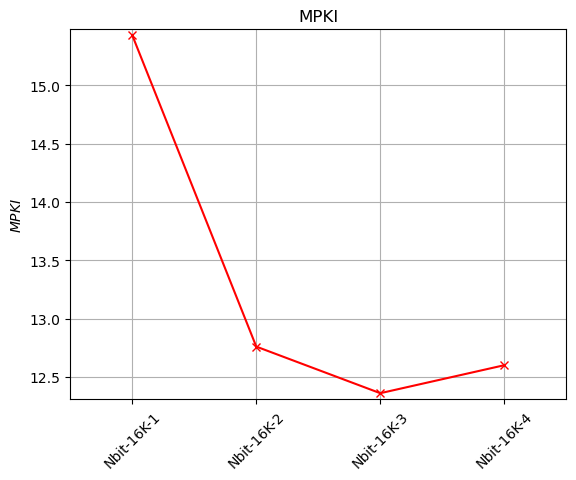
\includegraphics[width=\textwidth]{figures/5_3/401.bzip2.cslab_branch_preds_ref.out.png}
        \caption{401.bzip2}
        \label{fig:plot1}
    \end{subfigure}
    \hfill
    \begin{subfigure}[b]{0.45\textwidth}
        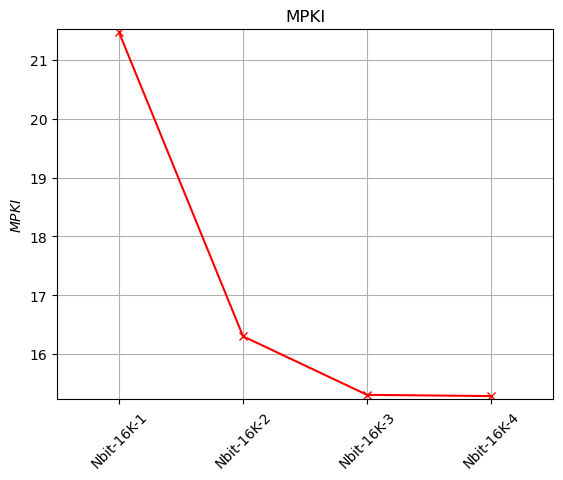
\includegraphics[width=\textwidth]{figures/5_3/403.gcc.cslab_branch_preds_ref.out.png}
        \caption{403.gcc}
        \label{fig:plot2}
    \end{subfigure}

    \vspace{0.5cm} % spacing between rows

    \begin{subfigure}[b]{0.45\textwidth}
        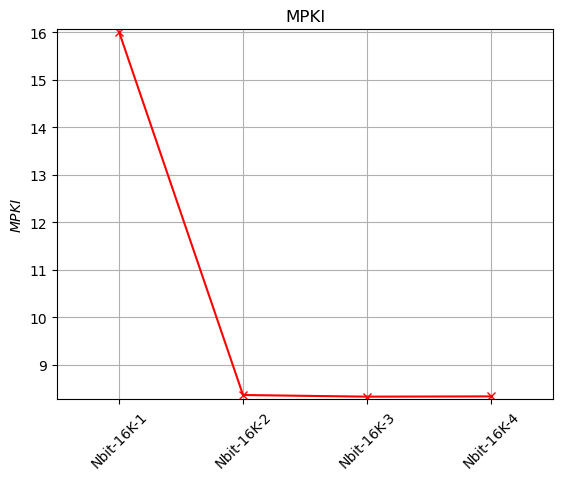
\includegraphics[width=\textwidth]{figures/5_3/410.bwaves.cslab_branch_preds_ref.out.png}
        \caption{410.bwaves}
        \label{fig:plot3}
    \end{subfigure}
    \hfill
    \begin{subfigure}[b]{0.45\textwidth}
        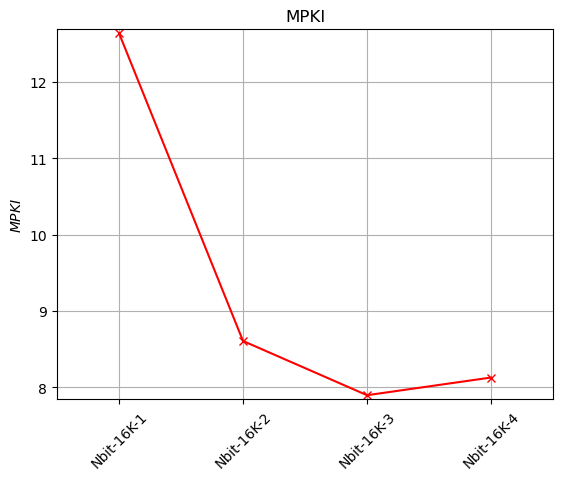
\includegraphics[width=\textwidth]{figures/5_3/416.gamess.cslab_branch_preds_ref.out.png}
        \caption{416.gamess}
        \label{fig:plot4}
    \end{subfigure}

    \vspace{0.5cm} % spacing between rows

    \begin{subfigure}[b]{0.45\textwidth}
        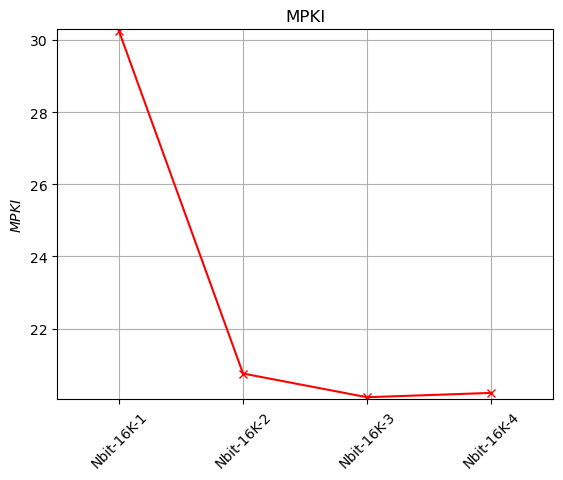
\includegraphics[width=\textwidth]{figures/5_3/429.mcf.cslab_branch_preds_ref.out.png}
        \caption{429.mcf}
        \label{fig:plot5}
    \end{subfigure}
    \hfill
    \begin{subfigure}[b]{0.45\textwidth}
        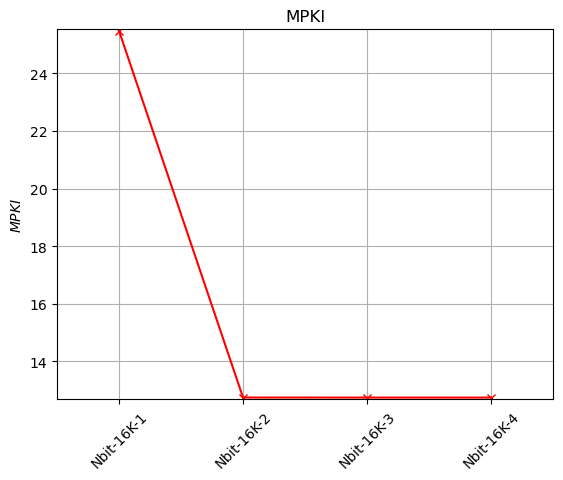
\includegraphics[width=\textwidth]{figures/5_3/433.milc.cslab_branch_preds_ref.out.png}
        \caption{433.milc}
        \label{fig:plot6}
    \end{subfigure}
    \vspace{0.5cm} 

    \caption{Branch Prediction Accuracy for Different N-bit Predictors}
    \label{fig:all_plots}
\end{figure}

\begin{figure}[H]
    \ContinuedFloat
    \centering

    \begin{subfigure}[b]{0.45\textwidth}
        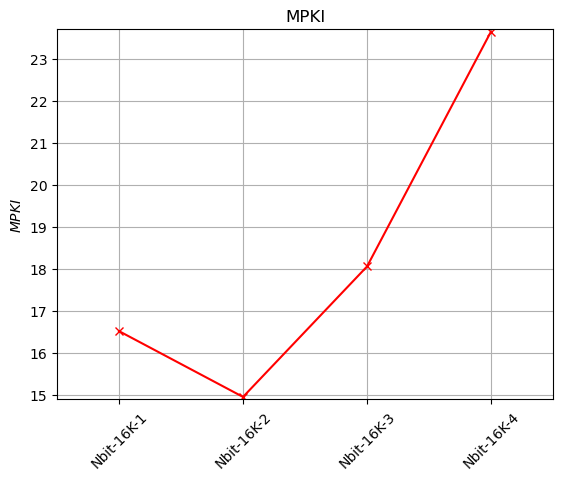
\includegraphics[width=\textwidth]{figures/5_3/435.gromacs.cslab_branch_preds_ref.out.png}
        \caption{435.gromacs}
        \label{fig:plot7}
    \end{subfigure}
    \hfill
    \begin{subfigure}[b]{0.45\textwidth}
        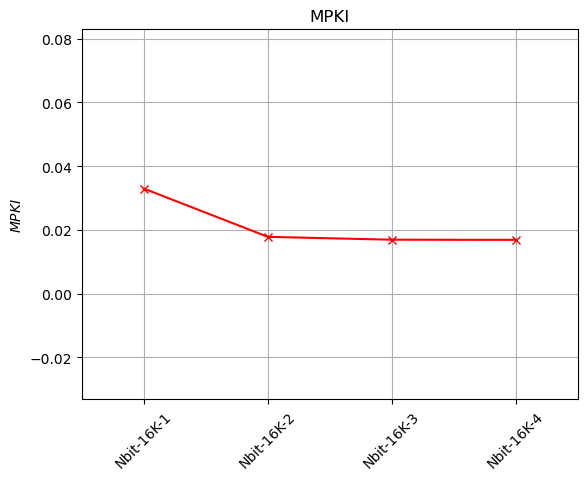
\includegraphics[width=\textwidth]{figures/5_3/436.cactusADM.cslab_branch_preds_ref.out.png}
        \caption{436.cactusADM}
        \label{fig:plot8}
    \end{subfigure}

    \vspace{0.5cm} % spacing between rows

    \begin{subfigure}[b]{0.45\textwidth}
        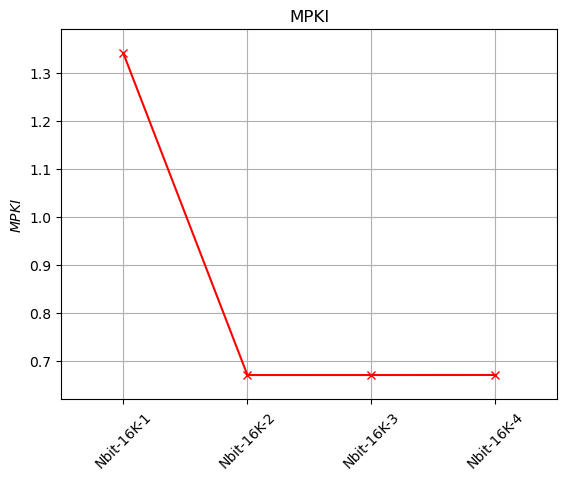
\includegraphics[width=\textwidth]{figures/5_3/437.leslie3d.cslab_branch_preds_ref.out.png}
        \caption{437.leslie3d}
        \label{fig:plot9}
    \end{subfigure}
    \hfill
    \begin{subfigure}[b]{0.45\textwidth}
        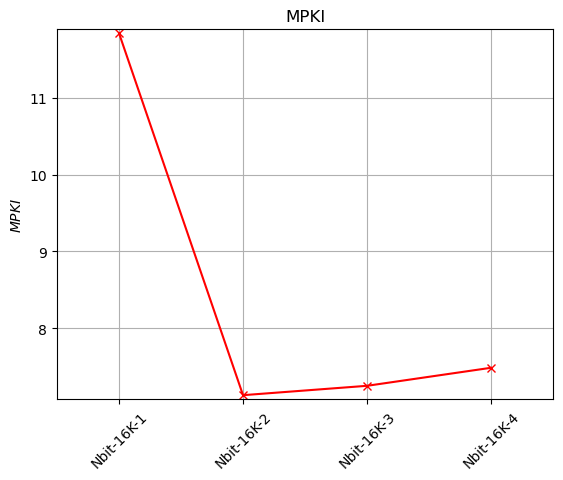
\includegraphics[width=\textwidth]{figures/5_3/450.soplex.cslab_branch_preds_ref.out.png}
        \caption{450.soplex}
        \label{fig:plot10}
    \end{subfigure}

    \vspace{0.5cm} % spacing between rows

    \begin{subfigure}[b]{0.45\textwidth}
        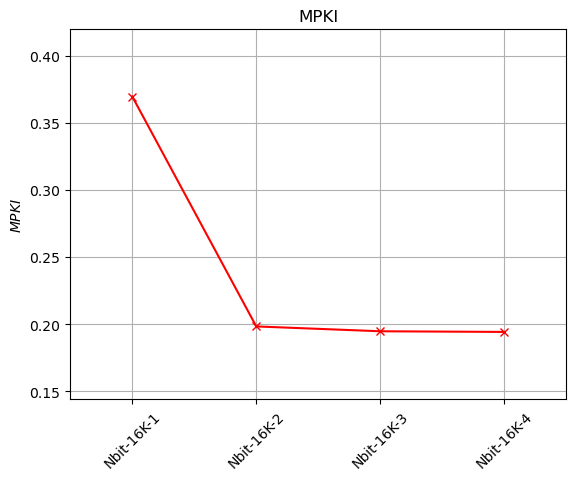
\includegraphics[width=\textwidth]{figures/5_3/456.hmmer.cslab_branch_preds_ref.out.png}
        \caption{456.hmmer}
        \label{fig:plot11}
    \end{subfigure}
    \hfill
    \begin{subfigure}[b]{0.45\textwidth}
        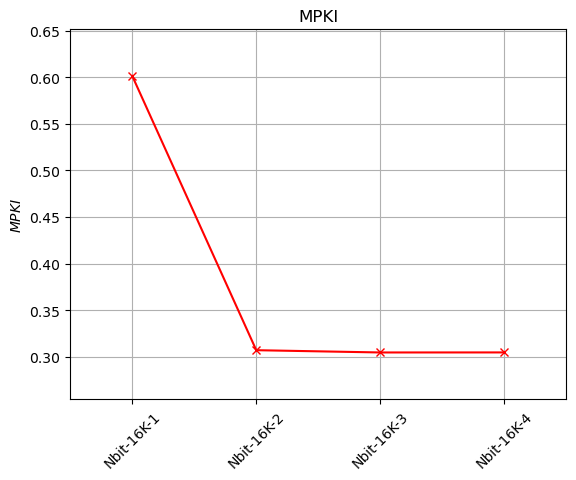
\includegraphics[width=\textwidth]{figures/5_3/459.GemsFDTD.cslab_branch_preds_ref.out.png}
        \caption{459.GemsFDTD}
        \label{fig:plot12}
    \end{subfigure}
    \vspace{0.5cm} 

    \caption{(continued)}
    \label{fig:nbits_part2}
\end{figure}

\begin{figure}[H]
    \ContinuedFloat
    \centering

    \begin{subfigure}[b]{0.45\textwidth}
        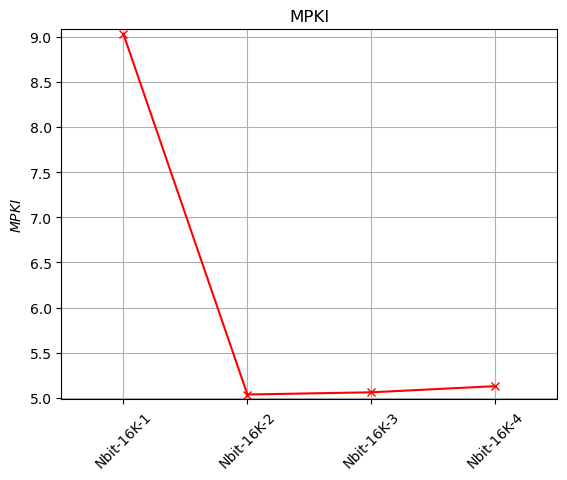
\includegraphics[width=\textwidth]{figures/5_3/464.h264ref.cslab_branch_preds_ref.out.png}
        \caption{464.h264ref}
        \label{fig:plot13}
    \end{subfigure}
    \hfill
    \begin{subfigure}[b]{0.45\textwidth}
        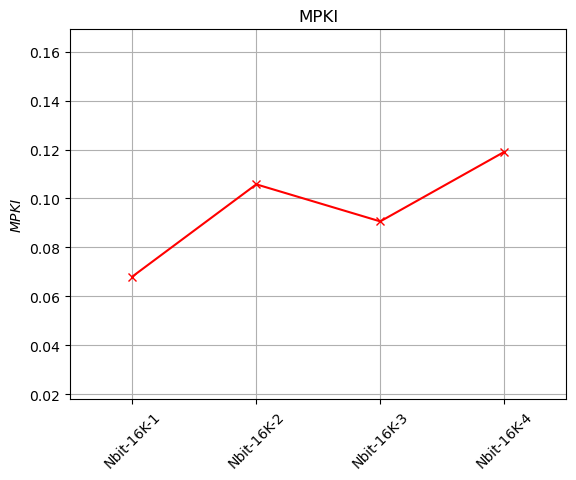
\includegraphics[width=\textwidth]{figures/5_3/470.lbm.cslab_branch_preds_ref.out.png}
        \caption{470.lbm}
        \label{fig:plot14}
    \end{subfigure}

    \vspace{0.5cm} % spacing between rows

    \begin{subfigure}[b]{0.45\textwidth}
        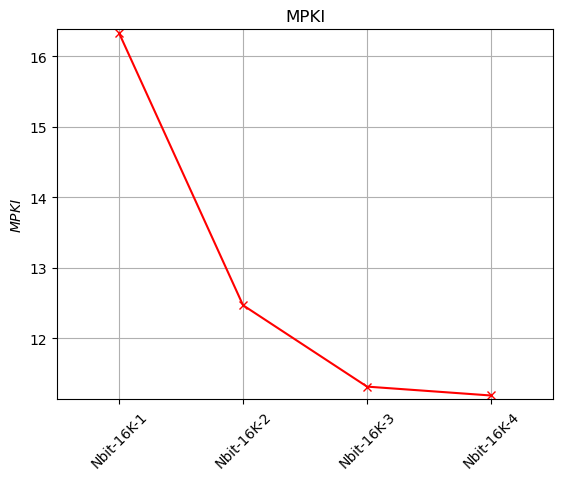
\includegraphics[width=\textwidth]{figures/5_3/471.omnetpp.cslab_branch_preds_ref.out.png}
        \caption{471.omnetpp}
        \label{fig:plot15}
    \end{subfigure}
    \hfill
    \begin{subfigure}[b]{0.45\textwidth}
        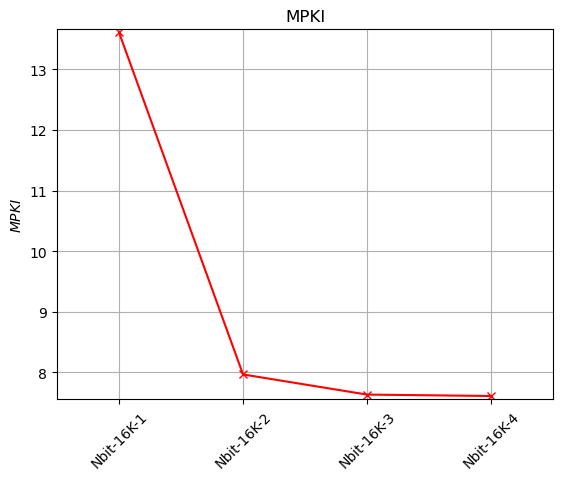
\includegraphics[width=\textwidth]{figures/5_3/483.xalancbmk.cslab_branch_preds_ref.out.png}
        \caption{483.xalancbmk}
        \label{fig:plot16}
    \end{subfigure}

    \vspace{0.5cm} 

    \caption{(continued)}
    \label{fig:nbits_part3}
\end{figure}

Υπολογίζουμε τον γεωμετρικό μέσο όρο του MPKI για κάθε benchmark και για κάθε n-bit predictor. 

\begin{figure}[H]
    \centering
    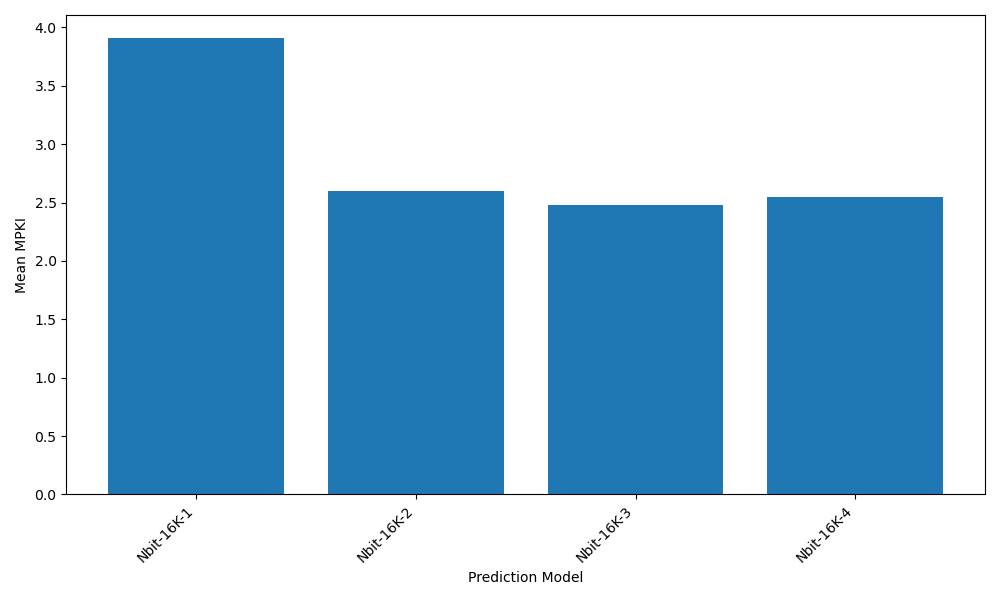
\includegraphics[width=0.65\textwidth]{figures/5_3/geom_mean.png}
    \caption{Geometric Mean MPKI for N-bit predictors}
    \label{fig:mean_mpkis}
\end{figure}

Παρατηρούμε από τα αποτελέσματα ότι ο Nbit-16K-1 predictor παρουσιάζει με διαφορά το υψηλότερο MPKI (3.90), ενώ οι υπόλοιποι τρεις (Nbit-16K-2, 3 και 4) κινούνται σε παρόμοια επίπεδα απόδοσης (2.60, 2.48 και 2.55 αντίστοιχα).

Επιλέγουμε τον \textbf{Nbit-16K-2}, καθώς προσφέρει ικανοποιητικές επιδόσεις με \textbf{χαμηλές απαιτήσεις σε επιπλέον υλικό (overhead)}. Αν και οι Nbit-16K-3 και Nbit-16K-4 εμφανίζουν ελαφρώς καλύτερο MPKI, η διαφορά είναι μικρή και δεν δικαιολογεί την αυξημένη πολυπλοκότητα.

\subsection{}
 Από το paper \textit{“Optimal 2-Bit Branch Predictors”} (R. Nair, 1995) βλέπουμε τα εξής πιθανά FSM:

 \begin{figure}[h!]
     \centering
     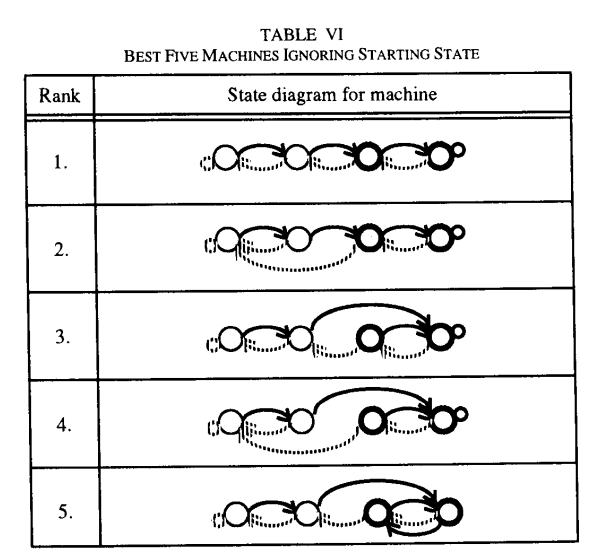
\includegraphics[width=0.5\linewidth]{figures/FMS.png}
     \caption{FSMs according to R. Nair.}
     \label{fig:enter-label}
 \end{figure}

 όπου με \textbf{bold} απεικονίζονται οι μεταβάσεις μετά από σωστή πρόβλεψη και \texttt{dotted} οι μεταβάσεις ύστερα από αποτυχημένη.

 Βασιζόμενοι σε αυτά τα διαγράμματα δημιουργούμε τους αντίστοιχους predictors στο αρχείο branch\_predictor.h:
 \begin{lstlisting}[style=cppstyle]
 class TwobitPredictor_FSM2 : public BranchPredictor
 {
 public:
     TwobitPredictor_FSM2(unsigned index_bits_ = 14, unsigned cntr_bits_ = 2)
     \\same as before ...

     virtual void update(bool predicted, bool actual, ADDRINT ip, ADDRINT target) {
         unsigned int ip_table_index = ip % table_entries;
         if (actual) {
             if (TABLE[ip_table_index] < COUNTER_MAX)
                 TABLE[ip_table_index]++;
         } else {
             if (TABLE[ip_table_index] == 2)
                 TABLE[ip_table_index] -= 2;
             else if (TABLE[ip_table_index] > 0)
                 TABLE[ip_table_index]--;
         }

         updateCounters(predicted, actual);
     };
 \end{lstlisting}
 Κατά αντίστοιχο τρόπο κατασκευάζουμε και τις υπόλοιπες κλάσεις τις οποίες μετά καλούμε στο cslab\_branch.cpp

 \begin{lstlisting}[style=cppstyle]
 new TwobitPredictor_FSM1();
 new TwobitPredictor_FSM2();
 new TwobitPredictor_FSM3();
 new TwobitPredictor_FSM4();
 new TwobitPredictor_FSM5();
 \end{lstlisting}

 \pagebreak
 Καταλήγουμε, λοιπόν, με τα εξής διαγραμμάτα:
 
 \begin{figure}[H]
     \centering
 
     \begin{subfigure}[b]{0.45\textwidth}
         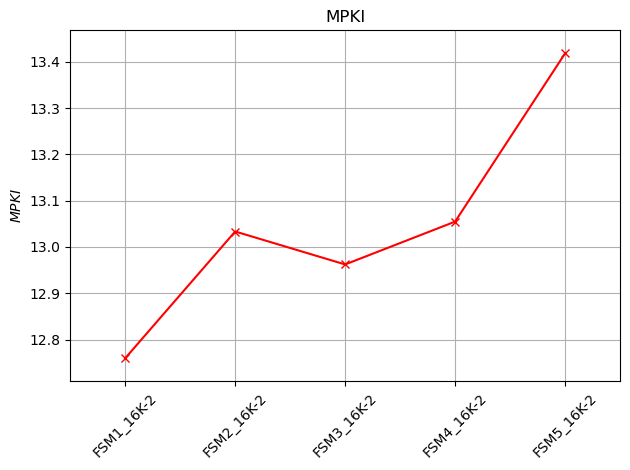
\includegraphics[width=\textwidth]{figures/5_3_b/401.bzip2.cslab_branch_preds_ref.out.png}
         \caption{401.bzip2}
         \label{fig:plot17}
     \end{subfigure}
     \hfill
     \begin{subfigure}[b]{0.45\textwidth}
         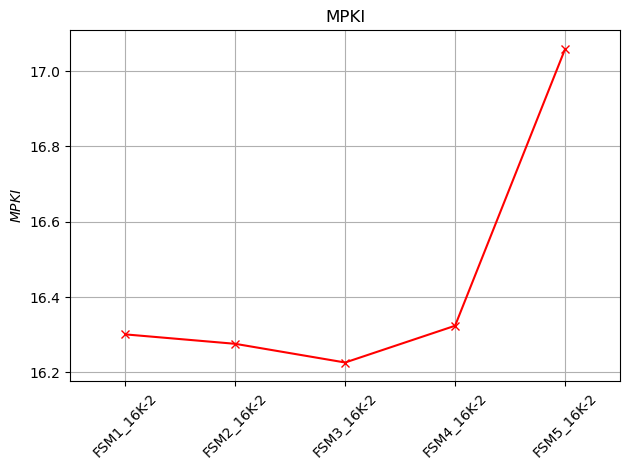
\includegraphics[width=\textwidth]{figures/5_3_b/403.gcc.cslab_branch_preds_ref.out.png}
         \caption{403.gcc}
         \label{fig:plot18}
     \end{subfigure}
 
     \vspace{0.5cm} % spacing between rows
 
     \begin{subfigure}[b]{0.45\textwidth}
         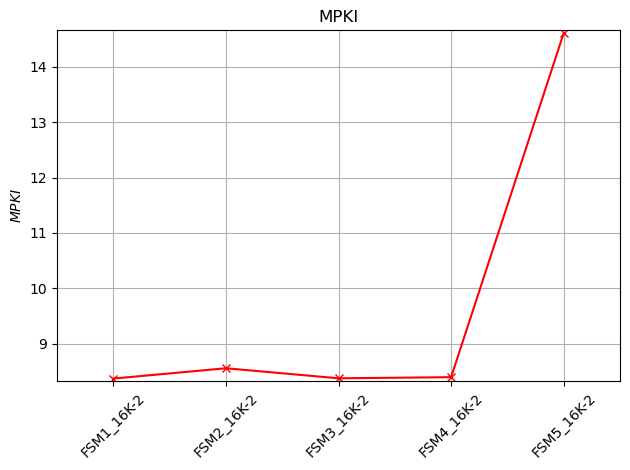
\includegraphics[width=\textwidth]{figures/5_3_b/410.bwaves.cslab_branch_preds_ref.out.png}
         \caption{410.bwaves}
         \label{fig:plot19}
     \end{subfigure}
     \hfill
     \begin{subfigure}[b]{0.45\textwidth}
         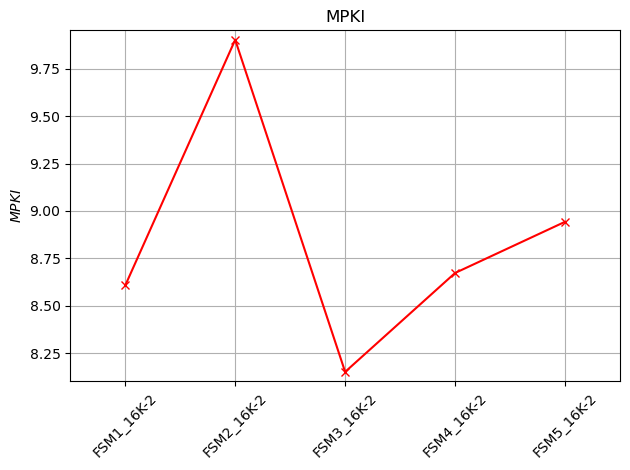
\includegraphics[width=\textwidth]{figures/5_3_b/416.gamess.cslab_branch_preds_ref.out.png}
         \caption{416.gamess}
         \label{fig:plot20}
     \end{subfigure}
 
     \vspace{0.5cm} % spacing between rows
 
     \begin{subfigure}[b]{0.45\textwidth}
         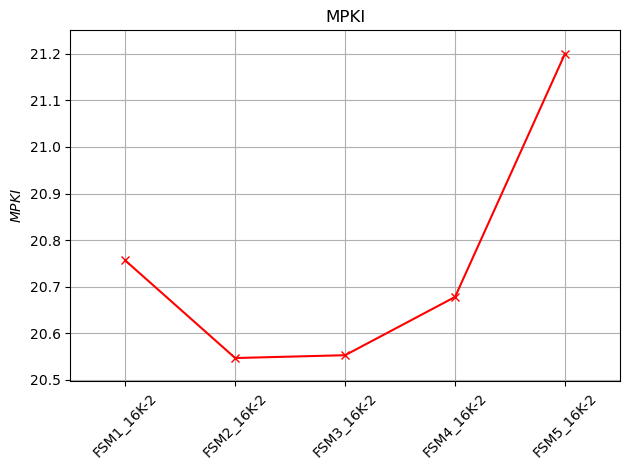
\includegraphics[width=\textwidth]{figures/5_3_b/429.mcf.cslab_branch_preds_ref.out.png}
         \caption{429.mcf}
         \label{fig:plot21}
     \end{subfigure}
     \hfill
     \begin{subfigure}[b]{0.45\textwidth}
         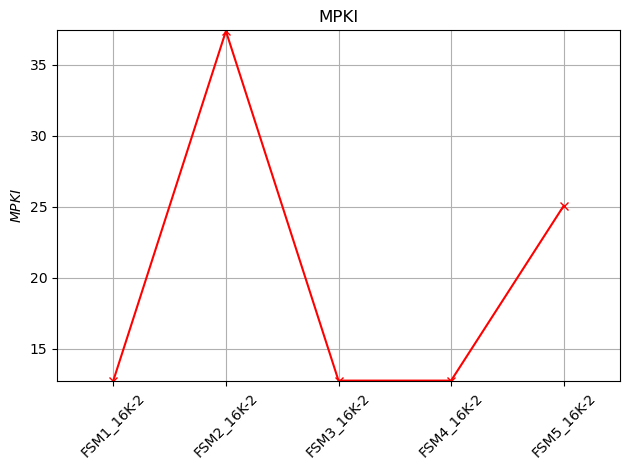
\includegraphics[width=\textwidth]{figures/5_3_b/433.milc.cslab_branch_preds_ref.out.png}
         \caption{433.milc}
         \label{fig:plot22}
     \end{subfigure}
     \vspace{0.5cm} 
 
     \caption{Branch Prediction Accuracy for Different N-bit Predictors}
     \label{fig:fsm}
 \end{figure}
 
 \begin{figure}[H]
     \ContinuedFloat
     \centering
 
     \begin{subfigure}[b]{0.45\textwidth}
         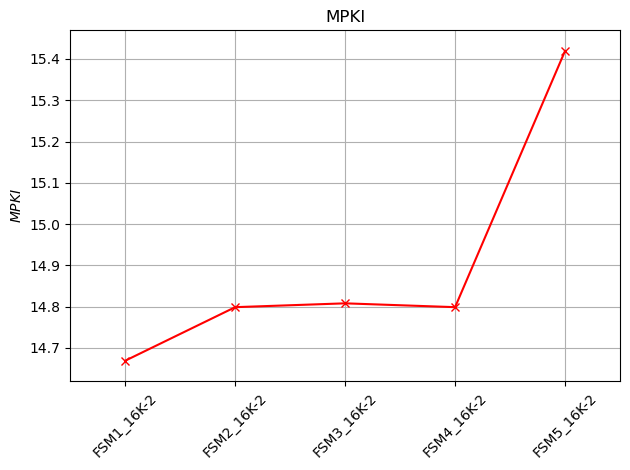
\includegraphics[width=\textwidth]{figures/5_3_b/435.gromacs.cslab_branch_preds_ref.out.png}
         \caption{435.gromacs}
         \label{fig:plot23}
     \end{subfigure}
     \hfill
     \begin{subfigure}[b]{0.45\textwidth}
         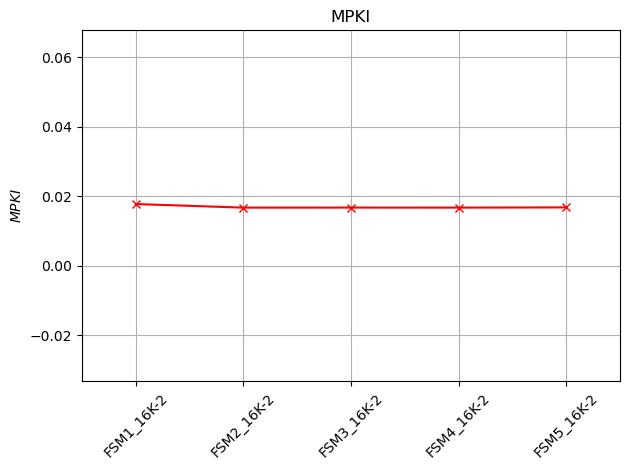
\includegraphics[width=\textwidth]{figures/5_3_b/436.cactusADM.cslab_branch_preds_ref.out.png}
         \caption{436.cactusADM}
         \label{fig:plot24}
     \end{subfigure}
 
     \vspace{0.5cm} % spacing between rows
 
     \begin{subfigure}[b]{0.45\textwidth}
         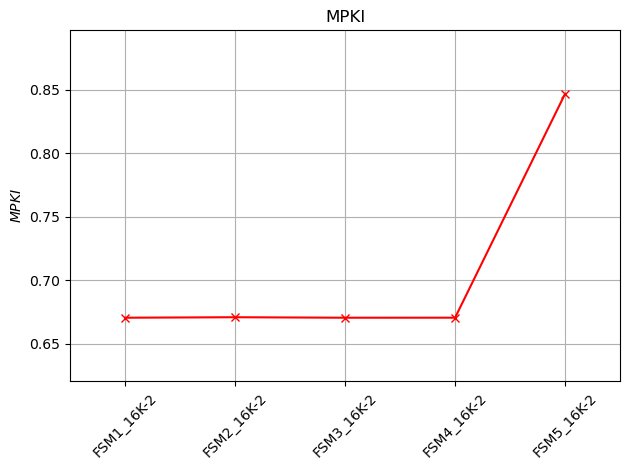
\includegraphics[width=\textwidth]{figures/5_3_b/437.leslie3d.cslab_branch_preds_ref.out.png}
         \caption{437.leslie3d}
         \label{fig:plot25}
     \end{subfigure}
     \hfill
     \begin{subfigure}[b]{0.45\textwidth}
         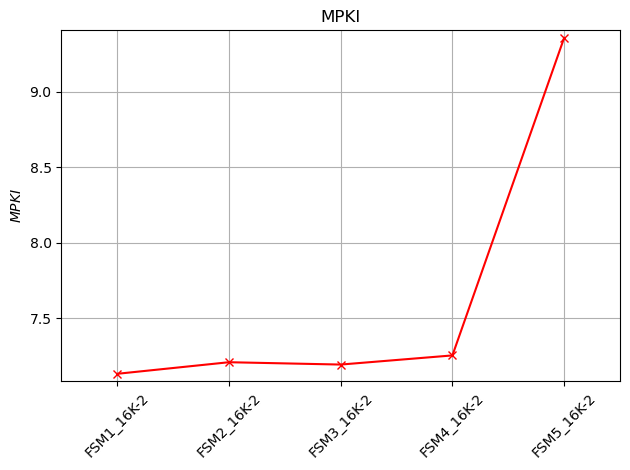
\includegraphics[width=\textwidth]{figures/5_3_b/450.soplex.cslab_branch_preds_ref.out.png}
         \caption{450.soplex}
         \label{fig:plot26}
     \end{subfigure}
 
     \vspace{0.5cm} % spacing between rows
 
     \begin{subfigure}[b]{0.45\textwidth}
         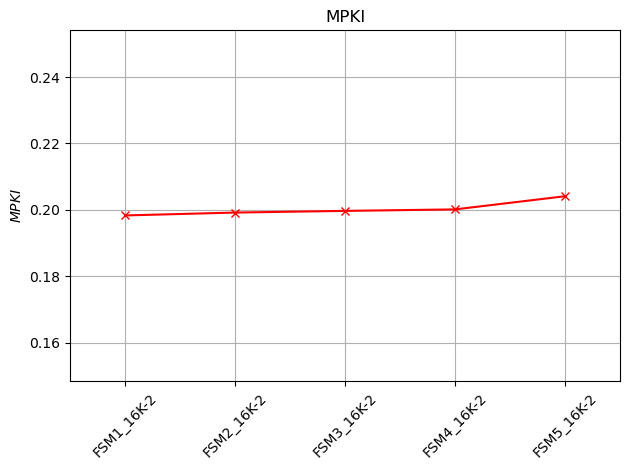
\includegraphics[width=\textwidth]{figures/5_3_b/456.hmmer.cslab_branch_preds_ref.out.png}
         \caption{456.hmmer}
         \label{fig:plot27}
     \end{subfigure}
     \hfill
     \begin{subfigure}[b]{0.45\textwidth}
         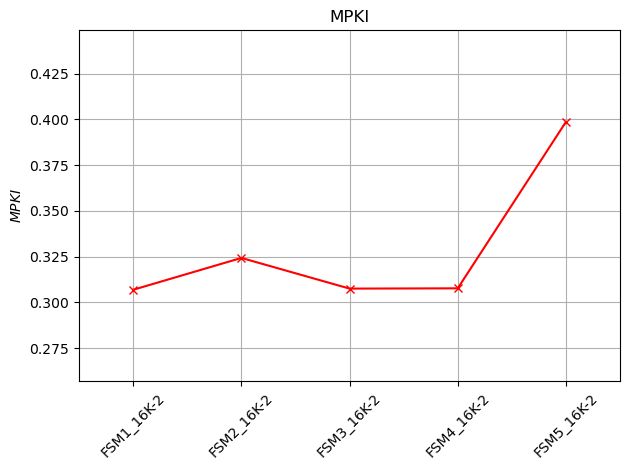
\includegraphics[width=\textwidth]{figures/5_3_b/459.GemsFDTD.cslab_branch_preds_ref.out.png}
         \caption{459.GemsFDTD}
         \label{fig:plot28}
     \end{subfigure}
     \vspace{0.5cm} 
 
     \caption{(continued)}
     \label{fig:fsm_part2}
 \end{figure}
 
 \begin{figure}[H]
     \ContinuedFloat
     \centering
 
     \begin{subfigure}[b]{0.45\textwidth}
         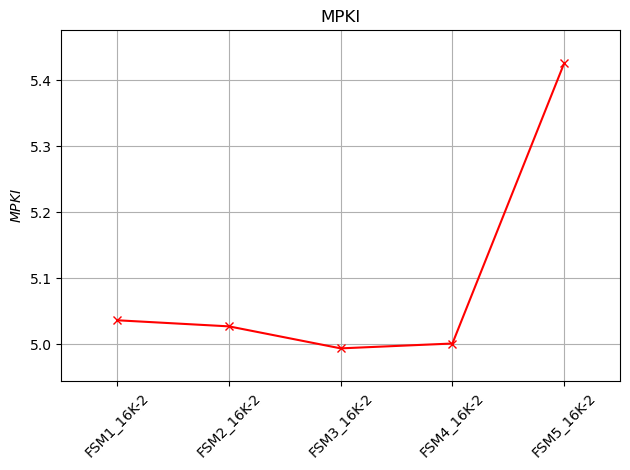
\includegraphics[width=\textwidth]{figures/5_3_b/464.h264ref.cslab_branch_preds_ref.out.png}
         \caption{464.h264ref}
         \label{fig:plot29}
     \end{subfigure}
     \hfill
     \begin{subfigure}[b]{0.45\textwidth}
         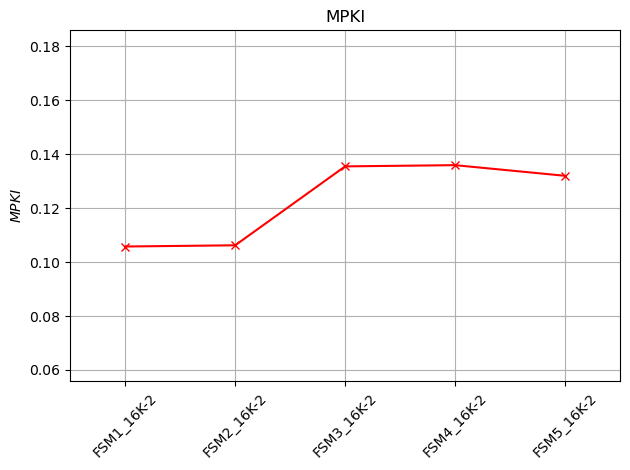
\includegraphics[width=\textwidth]{figures/5_3_b/470.lbm.cslab_branch_preds_ref.out.png}
         \caption{470.lbm}
         \label{fig:plot30}
     \end{subfigure}
 
     \vspace{0.5cm} % spacing between rows
 
     \begin{subfigure}[b]{0.45\textwidth}
         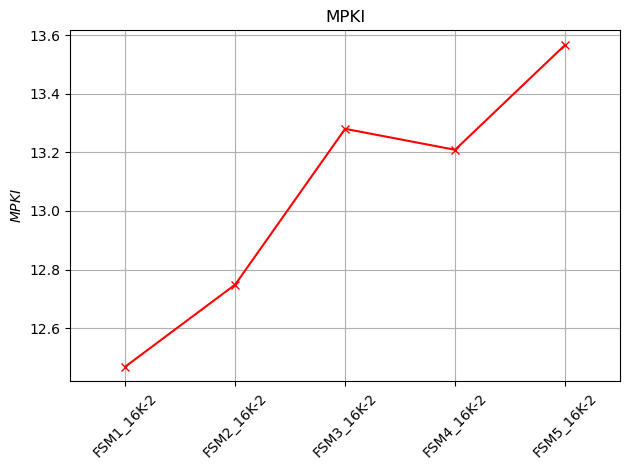
\includegraphics[width=\textwidth]{figures/5_3_b/471.omnetpp.cslab_branch_preds_ref.out.png}
         \caption{471.omnetpp}
         \label{fig:plot31}
     \end{subfigure}
     \hfill
     \begin{subfigure}[b]{0.45\textwidth}
         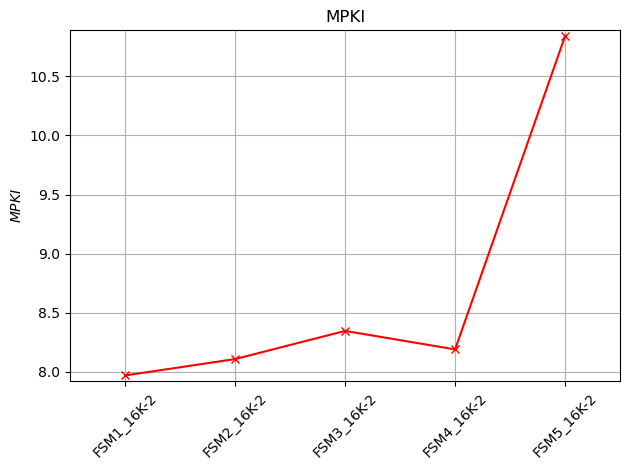
\includegraphics[width=\textwidth]{figures/5_3_b/483.xalancbmk.cslab_branch_preds_ref.out.png}
         \caption{483.xalancbmk}
         \label{fig:plot32}
     \end{subfigure}
 
     \vspace{0.5cm} 
 
     \caption{(continued)}
     \label{fig:fsm_part3}
 \end{figure}


 Υπολογίζουμε τον γεωμετρικό μέσο όρο του MPKI για κάθε benchmark και για κάθε FSM model. 

 \begin{figure}[H]
     \centering
     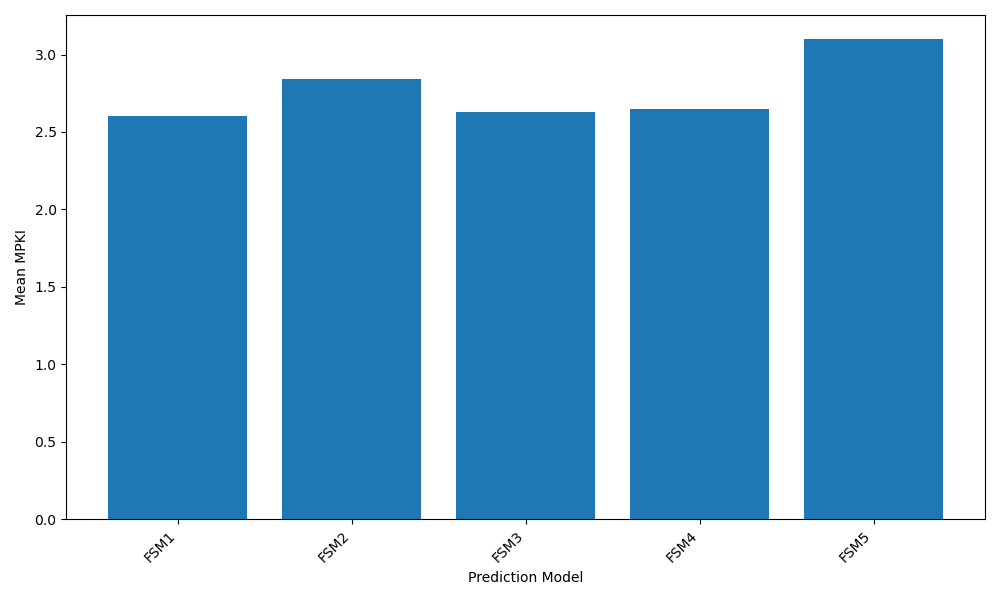
\includegraphics[width=0.65\textwidth]{figures/5_3_b/geom_mean.png}
     \caption{Geometric Mean MPKI for 16K-2 FSM models.}
     \label{fig:mean_mpkis_FSMs}
 \end{figure}

 Επιλέγουμε και πάλι τον απλό \textbf{Nbit-16K-2} predictor με \textbf{FSM1}, καθώς προσφέρει τις \textbf{βέλτιστες επιδόσεις} μεταξύ των εξεταζόμενων FSM και υλοποιείται με σχετικά απλό τρόπο, χρησιμοποιώντας έναν απλό saturating up-down counter.

 \subsection{}
 Προκειμένου να ορίσουμε το διαθέσιμο \textbf{hardware σε 32K bits}, θα πρέπει να ικανοποιείται η σχέση:
 \[
 \texttt{index\_bits} \times \texttt{cntr\_bits} = 32K
 \]
 Συνεπώς, τα δυνατά ζεύγη τιμών είναι:
 \[
 (15, 1),\quad (14, 2),\quad (13, 3)
 \]
 όπου το πρώτο στοιχείο κάθε ζεύγους αντιστοιχεί στον αριθμό των index bits και το δεύτερο στον αριθμό των bits του καταχωρητή (counter). Καλούμε, λοιπόν, τους εξής constructors στο cslab\_branch.cpp:


 \begin{lstlisting}[style=cppstyle]
     // 32K hardware
     new TwobitPredictor_FSM1();
     new TwobitPredictor_FSM2();
     new TwobitPredictor_FSM3();
     new TwobitPredictor_FSM4();
     new TwobitPredictor_FSM5();

     new NbitPredictor(15, 1);
     new NbitPredictor(13, 4);
 \end{lstlisting}

Και καταλήγουμε με τα εξής διαγράμματα:

\begin{figure}[H]
    \centering

    \begin{subfigure}[b]{0.45\textwidth}
        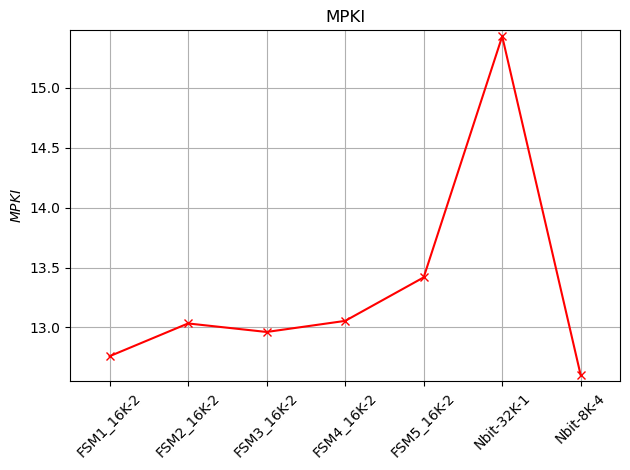
\includegraphics[width=\textwidth]{figures/5_3_c/401.bzip2.cslab_branch_preds_ref.out.png}
        \caption{401.bzip2}
        \label{fig:plot33}
    \end{subfigure}
    \hfill
    \begin{subfigure}[b]{0.45\textwidth}
        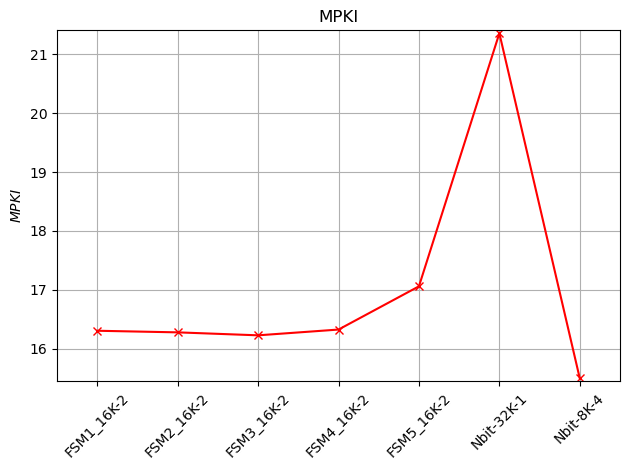
\includegraphics[width=\textwidth]{figures/5_3_c/403.gcc.cslab_branch_preds_ref.out.png}
        \caption{403.gcc}
        \label{fig:plot34}
    \end{subfigure}

    \vspace{0.5cm} % spacing between rows

    \begin{subfigure}[b]{0.45\textwidth}
        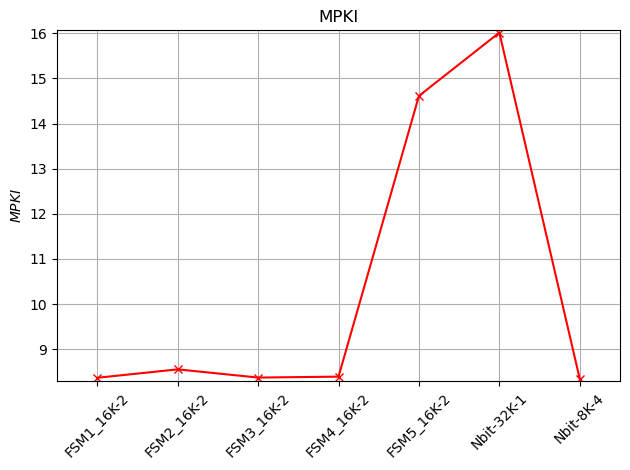
\includegraphics[width=\textwidth]{figures/5_3_c/410.bwaves.cslab_branch_preds_ref.out.png}
        \caption{410.bwaves}
        \label{fig:plot35}
    \end{subfigure}
    \hfill
    \begin{subfigure}[b]{0.45\textwidth}
        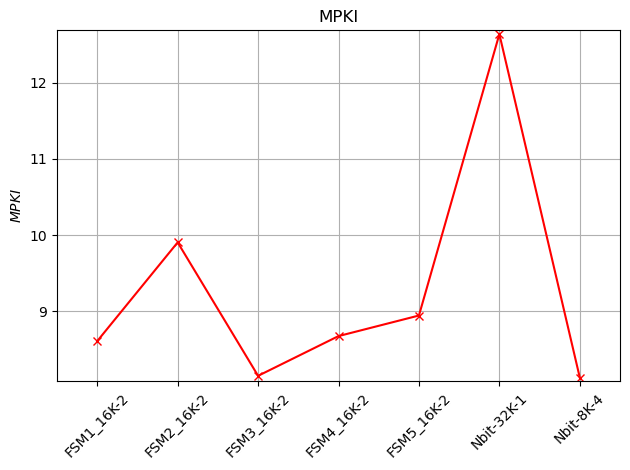
\includegraphics[width=\textwidth]{figures/5_3_c/416.gamess.cslab_branch_preds_ref.out.png}
        \caption{416.gamess}
        \label{fig:plot36}
    \end{subfigure}

    \vspace{0.5cm} % spacing between rows

    \caption{Branch Prediction Accuracy for Different 32K Predictors}
    \label{fig:32K}
\end{figure}

\begin{figure}[H]
    \centering
    \ContinuedFloat

    \begin{subfigure}[b]{0.45\textwidth}
        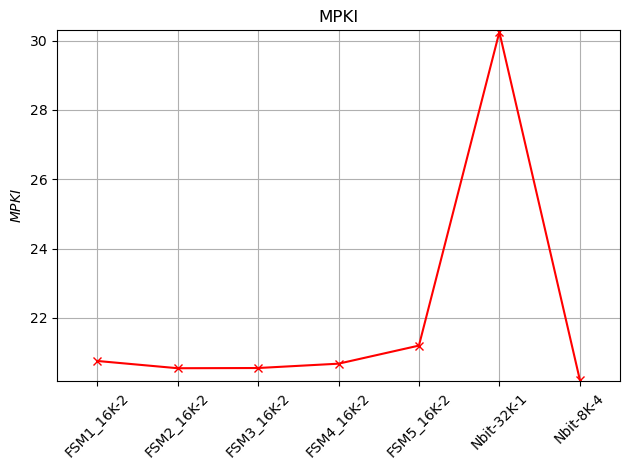
\includegraphics[width=\textwidth]{figures/5_3_c/429.mcf.cslab_branch_preds_ref.out.png}
        \caption{429.mcf}
        \label{fig:plot37}
    \end{subfigure}
    \hfill
    \begin{subfigure}[b]{0.45\textwidth}
        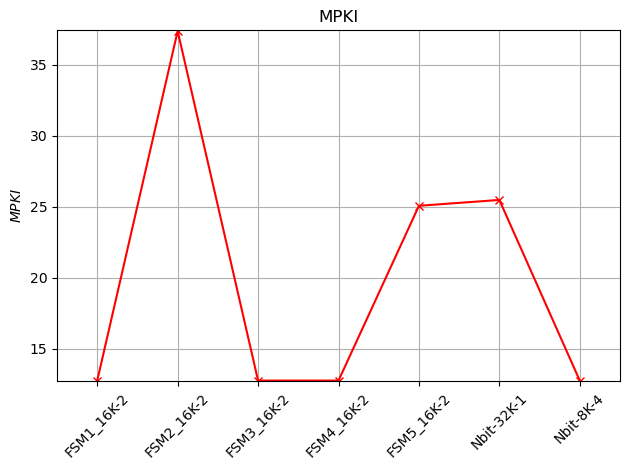
\includegraphics[width=\textwidth]{figures/5_3_c/433.milc.cslab_branch_preds_ref.out.png}
        \caption{433.milc}
        \label{fig:plot38}
    \end{subfigure}

    \vspace{0.5cm} % spacing between rows

    \begin{subfigure}[b]{0.45\textwidth}
        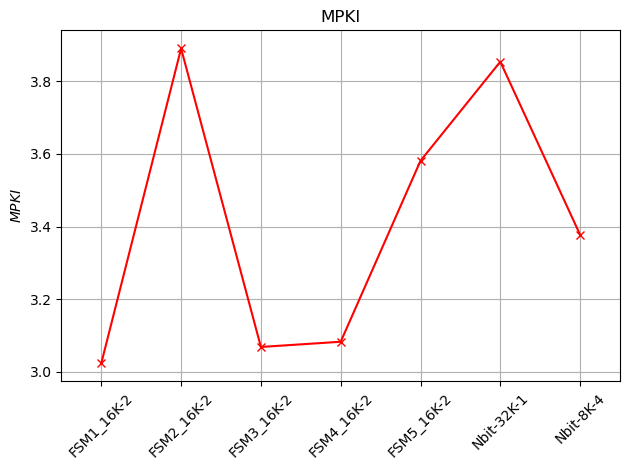
\includegraphics[width=\textwidth]{figures/5_3_c/435.gromacs.cslab_branch_preds_ref.out.png}
        \caption{435.gromacs}
        \label{fig:plot39}
    \end{subfigure}
    \hfill
    \begin{subfigure}[b]{0.45\textwidth}
        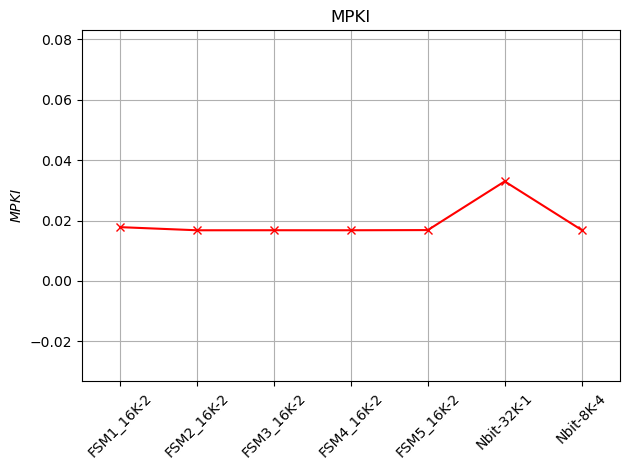
\includegraphics[width=\textwidth]{figures/5_3_c/436.cactusADM.cslab_branch_preds_ref.out.png}
        \caption{436.cactusADM}
        \label{fig:plot40}
    \end{subfigure}

    \vspace{0.5cm} % spacing between rows

    \begin{subfigure}[b]{0.45\textwidth}
        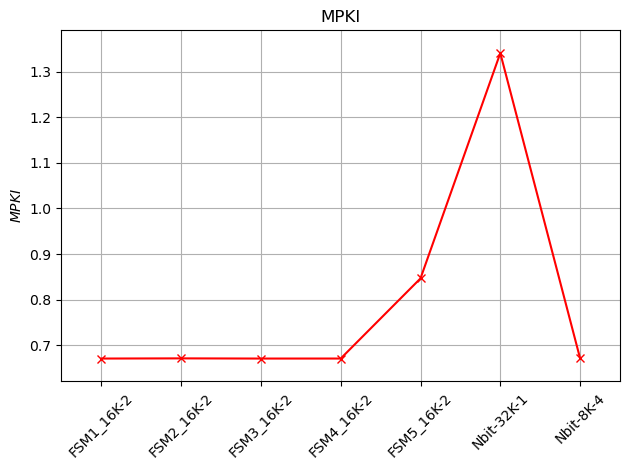
\includegraphics[width=\textwidth]{figures/5_3_c/437.leslie3d.cslab_branch_preds_ref.out.png}
        \caption{437.leslie3d}
        \label{fig:plot41}
    \end{subfigure}
    \hfill
    \begin{subfigure}[b]{0.45\textwidth}
        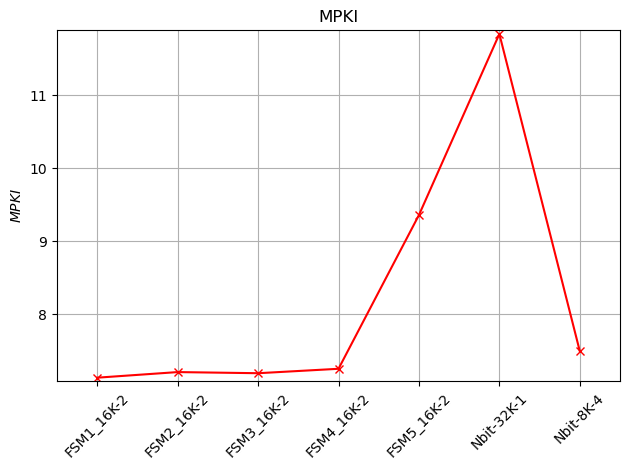
\includegraphics[width=\textwidth]{figures/5_3_c/450.soplex.cslab_branch_preds_ref.out.png}
        \caption{450.soplex}
        \label{fig:plot42}       
    \end{subfigure}
    \vspace{0.5cm} 
 
    \caption{(continued)}
    \label{fig:32K_part2}
\end{figure}

\begin{figure}
    \centering
    \ContinuedFloat

    \begin{subfigure}[b]{0.45\textwidth}
        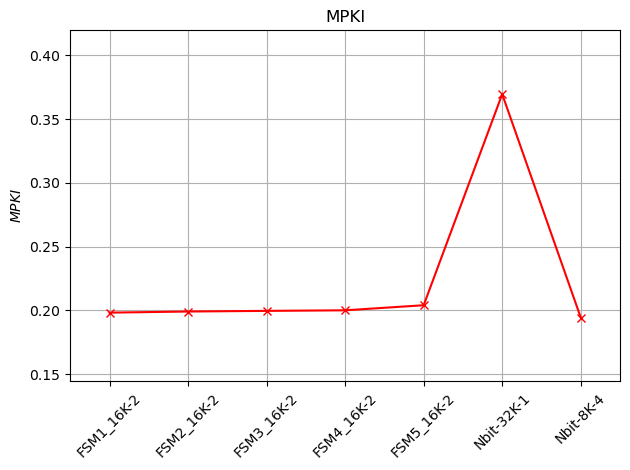
\includegraphics[width=\textwidth]{figures/5_3_c/456.hmmer.cslab_branch_preds_ref.out.png}
        \caption{456.hmmer}
        \label{fig:plot43}
    \end{subfigure}
    \hfill
    \begin{subfigure}[b]{0.45\textwidth}
        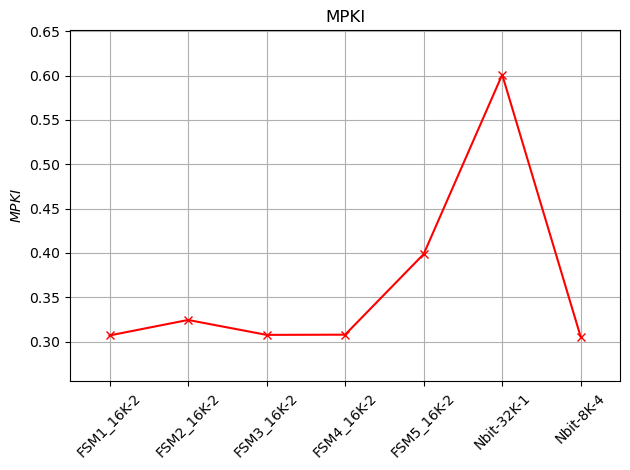
\includegraphics[width=\textwidth]{figures/5_3_c/459.GemsFDTD.cslab_branch_preds_ref.out.png}
        \caption{459.GemsFDTD}
        \label{fig:plot44}
    \end{subfigure}

    \vspace{0.5cm} % spacing between rows

    \begin{subfigure}[b]{0.45\textwidth}
        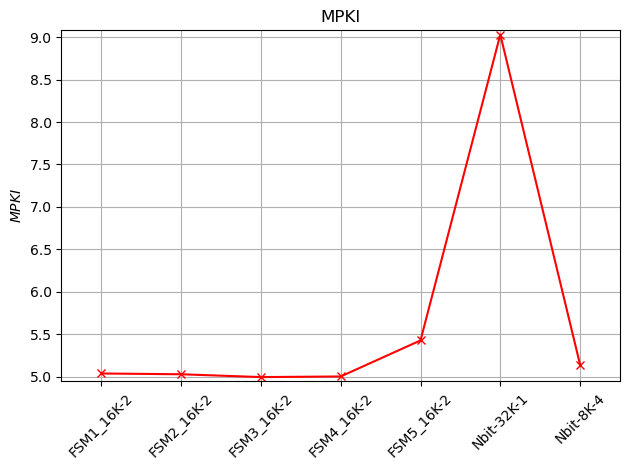
\includegraphics[width=\textwidth]{figures/5_3_c/464.h264ref.cslab_branch_preds_ref.out.png}
        \caption{464.h264ref}
        \label{fig:plot45}
    \end{subfigure}
    \hfill
    \begin{subfigure}[b]{0.45\textwidth}
        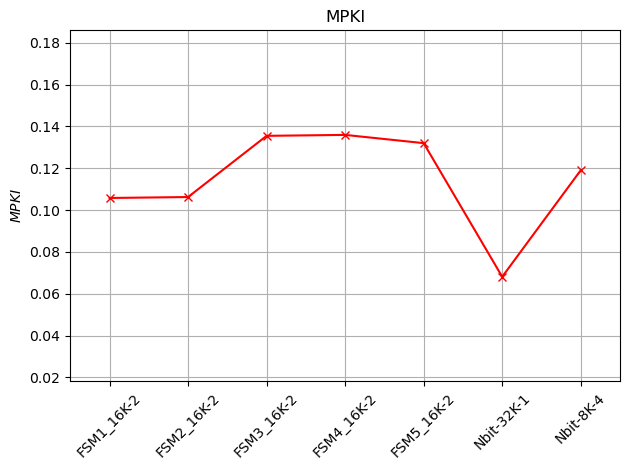
\includegraphics[width=\textwidth]{figures/5_3_c/470.lbm.cslab_branch_preds_ref.out.png}
        \caption{470.lbm}
        \label{fig:plot46}
    \end{subfigure}

    \vspace{0.5cm} % spacing between rows

    \begin{subfigure}[b]{0.45\textwidth}
        \includegraphics[width=\textwidth]{figures/5_3_c/471.omnetpp.cslab_branch_preds_ref.out.png}
        \caption{471.omnetpp}
        \label{fig:plot47}
    \end{subfigure}
    \hfill
    \begin{subfigure}[b]{0.45\textwidth}
        \includegraphics[width=\textwidth]{figures/5_3_c/483.xalancbmk.cslab_branch_preds_ref.out.png}
        \caption{483.xalancbmk}
        \label{fig:plot48}        
    \end{subfigure}
    \vspace{0.5cm}

    \caption{(continued)}
    \label{fig:32K_part3}
\end{figure}

\pagebreak

\begin{figure}[H]
    \centering
    \includegraphics[width=1\textwidth]{figures/5_3_c/geom_mean.png}
    \caption{Geometric Mean MPKI for 32K predictors}
    \label{fig:mean_mpkis_32K}
\end{figure}

Συνοψίζοντας, μεταξύ των εξεταζόμενων \textbf{Nbit predictors} με ίδιο συνολικό αποτύπωμα υλικού (\textbf{32K bits}), ο \textbf{Nbit-8K-4} παρουσιάζει τις \textbf{καλύτερες επιδόσεις} σε όρους MPKI, ξεπερνώντας ελαφρώς τον Nbit-16K-2. Επιπλέον, λόγω του μικρότερου αριθμού entries, προσφέρει και \textbf{μειωμένο latency}, γεγονός που τον καθιστά ταχύτερο στην πράξη. Αντιθέτως, ο Nbit-16K-2 εμφανίζει ελαφρώς \textbf{μικρότερη δυναμική κατανάλωση}, λόγω μικρότερου πλήθους toggled bits ανά update, όμως η διαφορά αυτή είναι περιορισμένη. Συνεπώς, για ένα σύστημα όπου προτεραιότητα έχουν οι επιδόσεις και η ταχύτητα, ο \textbf{Nbit-8K-4} αποτελεί την καταλληλότερη επιλογή.

\section{Μελέτη του ΒΤΒ}
\subsection*{BTB Predictors}

Οι BTB (Branch Target Buffer) predictors χρησιμοποιούνται για την πρόβλεψη του \textbf{διευθυνσιοδοτούμενου στόχου} (target address) ενός branch, σε περιπτώσεις όπου προβλέπεται ότι το branch θα εκτελεστεί (taken). Αντίθετα με τους κλασικούς branch predictors που απλώς αποφασίζουν αν το branch θα γίνει ή όχι, το BTB στοχεύει στο να επιταχύνει τη ροή εντολών προβλέποντας έγκαιρα \textbf{πού} θα μεταφερθεί ο έλεγχος.

Ένα BTB αποτελείται από έναν πίνακα εγγραφών (entries), όπου κάθε εγγραφή περιλαμβάνει:
\begin{itemize}
    \item Τη διεύθυνση της branch εντολής (PC),
    \item Την προβλεπόμενη διεύθυνση στόχου (target address),
    \item Ενδεχομένως metadata όπως valid bits ή ιστορικά στοιχεία.
\end{itemize}

Κατά την προσπέλαση, το BTB αναζητά μια αντιστοιχία μεταξύ της τρέχουσας διεύθυνσης εντολής και των αποθηκευμένων PC. Αν βρεθεί τέτοια εγγραφή και η πρόβλεψη είναι taken, τότε το pipeline μπορεί να προφορτώσει το target address χωρίς καθυστέρηση, μειώνοντας σημαντικά τα \textbf{penalties από mispredicted branches}.

Θα εξετάσουμε τις εξής περιπτώσεις BTB predictors:

\begin{table}[H]
    \centering
    \begin{tabular}{|c|c|}
    \hline
    \textbf{BTB Entries} & \textbf{BTB Associativity} \\
    \hline
    512 & 1, 2 \\
    \hline
    256 & 2, 4 \\
    \hline
    128 & 2, 4 \\
    \hline
    64  & 4, 8 \\
    \hline
    \end{tabular}
    \caption{BTB Configurations (Entries and Associativity)}
    \label{table:btb_configs}
\end{table}

Η υλοποίηση παραλείπεται για λόγους συντομίας.
Καλούμε τους παρακάτω BTB predictors στο cslab\_branch.cpp:
\begin{lstlisting}[style=cppstyle]
    VOID BTB()
    {
        btb_predictors.push_back(new BTBPredictor(512, 1));
        btb_predictors.push_back(new BTBPredictor(512, 2));
        btb_predictors.push_back(new BTBPredictor(256, 2));
        btb_predictors.push_back(new BTBPredictor(256, 4));
        btb_predictors.push_back(new BTBPredictor(128, 2));
        btb_predictors.push_back(new BTBPredictor(128, 4));
        btb_predictors.push_back(new BTBPredictor(64, 4));
        btb_predictors.push_back(new BTBPredictor(64, 8));
    }
\end{lstlisting}

Και καταλήγουμε με τα εξής διαγράμματα:
\begin{figure}[H]
    \centering

    \begin{subfigure}[b]{0.45\textwidth}
        \includegraphics[width=\textwidth]{figures/5_4/401.bzip2.cslab_branch_preds_ref.out.png}
        \caption{401.bzip2}
        \label{fig:plot49}
    \end{subfigure}
    \hfill
    \begin{subfigure}[b]{0.45\textwidth}
        \includegraphics[width=\textwidth]{figures/5_4/403.gcc.cslab_branch_preds_ref.out.png}
        \caption{403.gcc}
        \label{fig:plot50}
    \end{subfigure}

    \vspace{0.5cm} % spacing between rows

    \begin{subfigure}[b]{0.45\textwidth}
        \includegraphics[width=\textwidth]{figures/5_4/410.bwaves.cslab_branch_preds_ref.out.png}
        \caption{410.bwaves}
        \label{fig:plot51}
    \end{subfigure}
    \hfill
    \begin{subfigure}[b]{0.45\textwidth}
        \includegraphics[width=\textwidth]{figures/5_4/416.gamess.cslab_branch_preds_ref.out.png}
        \caption{416.gamess}
        \label{fig:plot52}
    \end{subfigure}

    \vspace{0.5cm} % spacing between rows

    \caption{BTB Predictors Accuracy for Different Configurations}
    \label{fig:btb}
\end{figure}

\begin{figure}[H]
    \centering
    \ContinuedFloat

    \begin{subfigure}[b]{0.45\textwidth}
        \includegraphics[width=\textwidth]{figures/5_4/429.mcf.cslab_branch_preds_ref.out.png}
        \caption{429.mcf}
        \label{fig:plot53}
    \end{subfigure}
    \hfill
    \begin{subfigure}[b]{0.45\textwidth}
        \includegraphics[width=\textwidth]{figures/5_4/433.milc.cslab_branch_preds_ref.out.png}
        \caption{433.milc}
        \label{fig:plot54}
    \end{subfigure}

    \vspace{0.5cm} % spacing between rows

    \begin{subfigure}[b]{0.45\textwidth}
        \includegraphics[width=\textwidth]{figures/5_4/435.gromacs.cslab_branch_preds_ref.out.png}
        \caption{435.gromacs}
        \label{fig:plot55}
    \end{subfigure}
    \hfill
    \begin{subfigure}[b]{0.45\textwidth}
        \includegraphics[width=\textwidth]{figures/5_4/436.cactusADM.cslab_branch_preds_ref.out.png}
        \caption{436.cactusADM}
        \label{fig:plot56}
    \end{subfigure}

    \vspace{0.5cm} % spacing between rows

    \begin{subfigure}[b]{0.45\textwidth}
        \includegraphics[width=\textwidth]{figures/5_4/437.leslie3d.cslab_branch_preds_ref.out.png}
        \caption{437.leslie3d}
        \label{fig:plot57}
    \end{subfigure}
    \hfill
    \begin{subfigure}[b]{0.45\textwidth}
        \includegraphics[width=\textwidth]{figures/5_4/450.soplex.cslab_branch_preds_ref.out.png}
        \caption{450.soplex}
        \label{fig:plot58}
    \end{subfigure}
    
    \vspace{0.5cm} % spacing between rows

    \caption{(continued)}
    \label{fig:btb_part2}
\end{figure}

\begin{figure}[H]
    \centering
    \ContinuedFloat

    \begin{subfigure}[b]{0.45\textwidth}
        \includegraphics[width=\textwidth]{figures/5_4/456.hmmer.cslab_branch_preds_ref.out.png}
        \caption{456.hmmer}
        \label{fig:plot59}
    \end{subfigure}
    \hfill
    \begin{subfigure}[b]{0.45\textwidth}
        \includegraphics[width=\textwidth]{figures/5_4/459.GemsFDTD.cslab_branch_preds_ref.out.png}
        \caption{459.GemsFDTD}
        \label{fig:plot60}
    \end{subfigure}

    \vspace{0.5cm} % spacing between rows

    \begin{subfigure}[b]{0.45\textwidth}
        \includegraphics[width=\textwidth]{figures/5_4/464.h264ref.cslab_branch_preds_ref.out.png}
        \caption{464.h264ref}
        \label{fig:plot61}
    \end{subfigure}
    \hfill
    \begin{subfigure}[b]{0.45\textwidth}
        \includegraphics[width=\textwidth]{figures/5_4/470.lbm.cslab_branch_preds_ref.out.png}
        \caption{470.lbm}
        \label{fig:plot62}
    \end{subfigure}

    \vspace{0.5cm} % spacing between rows

    \begin{subfigure}[b]{0.45\textwidth}
        \includegraphics[width=\textwidth]{figures/5_4/471.omnetpp.cslab_branch_preds_ref.out.png}
        \caption{471.omnetpp}
        \label{fig:plot63}
    \end{subfigure}
    \hfill
    \begin{subfigure}[b]{0.45\textwidth}
        \includegraphics[width=\textwidth]{figures/5_4/483.xalancbmk.cslab_branch_preds_ref.out.png}
        \caption{483.xalancbmk}
        \label{fig:plot64}
    \end{subfigure}
    
    \vspace{0.5cm} % spacing between rows

    \caption{(continued)}
    \label{fig:btb_part3}
\end{figure}

\begin{figure}[H]
    \centering
    \includegraphics[width=1\textwidth]{figures/5_4/geom_mean.png}
    \caption{Geometric Mean MPKI for BTB predictors}
    \label{fig:mean_mpkis_BTBs}
\end{figure}

Η απόδοση των διαφόρων διαμορφώσεων BTB επηρεάζεται από τον αριθμό των εγγραφών (entries) και την associativity, καθώς αυτά καθορίζουν την ικανότητα αποθήκευσης και γρήγορης ανάκτησης διευθύνσεων στόχων διακλαδώσεων.

\textbf{Αριθμός Εγγραφών (Entries):} Όσο περισσότερες οι εγγραφές, τόσο περισσότερες μοναδικές διακλαδώσεις μπορεί να αποθηκεύσει ο BTB, μειώνοντας τα \textit{capacity misses}—δηλαδή, αστοχίες λόγω ανεπαρκούς χώρου.

\textbf{Associativity:} Ορίζει πόσες διαφορετικές διακλαδώσεις μπορούν να αντιστοιχηθούν στην ίδια ομάδα (set). Υψηλότερη associativity μειώνει τα \textit{conflict misses}, δηλαδή αστοχίες που προκύπτουν από σύγκρουση πολλών διακλαδώσεων στον ίδιο περιορισμένο αριθμό θέσεων.

\vspace{0.3cm} \textbf{Επίδραση της Associativity (σταθερός αριθμός entries):} \begin{itemize} \item 512-1 (4.10) → 512-2 (3.94): Μεγάλη βελτίωση από associativity 1 σε 2. \item 256-2 (3.98) → 256-4 (3.92): Μικρή αλλά μετρήσιμη βελτίωση. \item 128-2 (4.09) → 128-4 (3.94): Σημαντική βελτίωση. \item 64-4 (4.01) → 64-8 (3.93): Αξιοσημείωτη βελτίωση. \end{itemize}

\textbf{Επίδραση του Αριθμού Εγγραφών (σταθερή associativity):} \begin{itemize} \item Associativity 2: 128-2 (4.09) → 256-2 (3.98) → 512-2 (3.94) \item Associativity 4: 64-4 (4.01) → 128-4 (3.94) → 256-4 (3.92) \end{itemize}

\vspace{0.3cm} \textbf{Παρατηρήσεις:} \begin{itemize} \item Οι καλύτερες επιδόσεις (χαμηλότερο MPKI) εμφανίζονται στις διαμορφώσεις: 256-4 (3.92), 64-8 (3.93), 512-2 (3.94), και 128-4 (3.94). \item Η αύξηση μόνο των entries χωρίς ανάλογη αύξηση στην associativity (π.χ., 512-1) οδηγεί σε χαμηλή απόδοση λόγω conflict misses. \item Η αύξηση της associativity αποδεικνύεται σταθερά ευεργετική για την απόδοση. \end{itemize}

\vspace{0.3cm} \textbf{Επιλογή Διαμόρφωσης:}

Η επιλογή του βέλτιστου BTB εξαρτάται από τον συμβιβασμό ανάμεσα στην απόδοση (χαμηλό MPKI) και το κόστος υλοποίησης (σε μέγεθος και πολυπλοκότητα). Ένας πρακτικός δείκτης μεγέθους είναι το γινόμενο \textit{Entries × Associativity}:

\begin{itemize} \item \textbf{256-4}: Καλύτερη απόδοση (3.92 MPKI), μέγεθος 256×4=1024. \item \textbf{64-8}: Ανταγωνιστική απόδοση (3.93 MPKI), μικρότερο μέγεθος 64×8=512. \item \textbf{128-4}: Εξίσου καλή απόδοση (3.94 MPKI), ίδιο μέγεθος με το 64-8. \item \textbf{512-2}: Καλή απόδοση (3.94 MPKI), αλλά μεγαλύτερο μέγεθος 512×2=1024. \end{itemize}

\textbf{Συμπέρασμα:}
Παρόλο που η διαμόρφωση \textbf{256-4} προσφέρει την απόλυτα καλύτερη απόδοση, οι διαμορφώσεις \textbf{64-8} και \textbf{128-4} αποτελούν εξαιρετικές εναλλακτικές με παρόμοια απόδοση και σημαντικά μικρότερο υπολογιζόμενο μέγεθος. Συνεπώς, για έναν καλό συμβιβασμό ανάμεσα σε απόδοση και κόστος υλικού, προτείνεται η διαμόρφωση \textbf{64-8} ή \textbf{128-4}.
\vspace{0.3cm}
\noindent \textbf{Τελική Επιλογή:} Το \textbf{BTB-256-4} αποτελεί την καλύτερη ισορροπία μεταξύ επίδοσης και κόστους υλοποίησης.

\section{Μελέτη του RAS}
Η \textbf{Return Address Stack (RAS)} είναι ένας εξειδικευμένος μηχανισμός πρόβλεψης διακλαδώσεων που χρησιμοποιείται για την πρόβλεψη διευθύνσεων επιστροφής από υπορουτίνες (function calls). Κάθε φορά που εκτελείται μία εντολή \texttt{call}, η διεύθυνση επιστροφής αποθηκεύεται στη στοίβα της RAS. Όταν αργότερα εκτελείται μία \texttt{return}, η προβλεπόμενη διεύθυνση λαμβάνεται από την κορυφή της στοίβας. Αυτός ο μηχανισμός είναι εξαιρετικά αποτελεσματικός, καθώς οι \texttt{return} εντολές εμφανίζονται συχνά και η αλληλουχία \texttt{call-return} διατηρείται κατά κανόνα με μεγάλη ακρίβεια.

Η απόδοση της RAS επηρεάζεται κυρίως από το μέγεθός της, δηλαδή από τον αριθμό των διευθύνσεων που μπορεί να κρατήσει. Μια μικρή RAS μπορεί να "ξεχειλίσει" όταν υπάρχουν πολλές εμφωλευμένες κλήσεις (nested calls), οδηγώντας σε λάθος πρόβλεψη. Αντίθετα, μια πολύ μεγάλη RAS μπορεί να καταναλώνει περιττούς πόρους χωρίς σημαντική βελτίωση στην απόδοση.

\vspace{0.3cm} \textbf{Δοκιμασμένες διαμορφώσεις RAS:}

\begin{lstlisting}[style=cppstyle]
    VOID InitRas()
    {
        for (UINT32 i = 4; i <= 64; i*=2) {
            ras_vec.push_back(new RAS(i));
            if (i == 32)
                ras_vec.push_back(new RAS(48));
    
            }
    }
\end{lstlisting}

Και καταλήγουμε με τα εξής διαγράμματα:

\begin{figure}[H]
    \centering

    \begin{subfigure}[b]{0.45\textwidth}
        \includegraphics[width=\textwidth]{figures/5_5/401.bzip2.cslab_branch_preds_ref.out.png}
        \caption{401.bzip2}
        \label{fig:plot65}
    \end{subfigure}
    \hfill
    \begin{subfigure}[b]{0.45\textwidth}
        \includegraphics[width=\textwidth]{figures/5_5/403.gcc.cslab_branch_preds_ref.out.png}
        \caption{403.gcc}
        \label{fig:plot66}
    \end{subfigure}

    \vspace{0.5cm} % spacing between rows

    \caption{RAS Accuracy for Different Configurations}
    \label{fig:ras}
\end{figure}

\begin{figure}[H]
    \centering
    \ContinuedFloat

    \begin{subfigure}[b]{0.45\textwidth}
        \includegraphics[width=\textwidth]{figures/5_5/410.bwaves.cslab_branch_preds_ref.out.png}
        \caption{410.bwaves}
        \label{fig:plot67}
    \end{subfigure}
    \hfill
    \begin{subfigure}[b]{0.45\textwidth}
        \includegraphics[width=\textwidth]{figures/5_5/416.gamess.cslab_branch_preds_ref.out.png}
        \caption{416.gamess}
        \label{fig:plot68}
    \end{subfigure}

    \vspace{0.5cm} % spacing between rows

    \begin{subfigure}[b]{0.45\textwidth}
        \includegraphics[width=\textwidth]{figures/5_5/429.mcf.cslab_branch_preds_ref.out.png}
        \caption{429.mcf}
        \label{fig:plot69}
    \end{subfigure}
    \hfill
    \begin{subfigure}[b]{0.45\textwidth}
        \includegraphics[width=\textwidth]{figures/5_5/433.milc.cslab_branch_preds_ref.out.png}
        \caption{433.milc}
        \label{fig:plot70}
    \end{subfigure}

    \vspace{0.5cm} % spacing between rows

    \begin{subfigure}[b]{0.45\textwidth}
        \includegraphics[width=\textwidth]{figures/5_5/435.gromacs.cslab_branch_preds_ref.out.png}
        \caption{435.gromacs}
        \label{fig:plot71}
    \end{subfigure}
    \hfill
    \begin{subfigure}[b]{0.45\textwidth}
        \includegraphics[width=\textwidth]{figures/5_5/436.cactusADM.cslab_branch_preds_ref.out.png}
        \caption{436.cactusADM}
        \label{fig:plot72}
    \end{subfigure}

    \vspace{0.5cm} % spacing between rows

    \caption{(continued)}
    \label{fig:ras_part2}
\end{figure}

\begin{figure}[H]
    \centering
    \ContinuedFloat

    \begin{subfigure}[b]{0.45\textwidth}
        \includegraphics[width=\textwidth]{figures/5_5/437.leslie3d.cslab_branch_preds_ref.out.png}
        \caption{437.leslie3d}
        \label{fig:plot73}
    \end{subfigure}
    \hfill
    \begin{subfigure}[b]{0.45\textwidth}
        \includegraphics[width=\textwidth]{figures/5_5/450.soplex.cslab_branch_preds_ref.out.png}
        \caption{450.soplex}
        \label{fig:plot74}
    \end{subfigure}

    \vspace{0.5cm} % spacing between rows

    \begin{subfigure}[b]{0.45\textwidth}
        \includegraphics[width=\textwidth]{figures/5_5/456.hmmer.cslab_branch_preds_ref.out.png}
        \caption{456.hmmer}
        \label{fig:plot75}
    \end{subfigure}
    \hfill
    \begin{subfigure}[b]{0.45\textwidth}
        \includegraphics[width=\textwidth]{figures/5_5/459.GemsFDTD.cslab_branch_preds_ref.out.png}
        \caption{459.GemsFDTD}
        \label{fig:plot76}
    \end{subfigure}

    \vspace{0.5cm} % spacing between rows

    \begin{subfigure}[b]{0.45\textwidth}
        \includegraphics[width=\textwidth]{figures/5_5/464.h264ref.cslab_branch_preds_ref.out.png}
        \caption{464.h264ref}
        \label{fig:plot77}
    \end{subfigure}
    \hfill
    \begin{subfigure}[b]{0.45\textwidth}
        \includegraphics[width=\textwidth]{figures/5_5/470.lbm.cslab_branch_preds_ref.out.png}
        \caption{470.lbm}
        \label{fig:plot78}
    \end{subfigure}

    \vspace{0.5cm} % spacing between rows

    \caption{(continued)}
    \label{fig:ras_part3}
\end{figure}

\begin{figure}[H]
    \centering
    \ContinuedFloat

    \begin{subfigure}[b]{0.45\textwidth}
        \includegraphics[width=\textwidth]{figures/5_5/471.omnetpp.cslab_branch_preds_ref.out.png}
        \caption{471.omnetpp}
        \label{fig:plot79}
    \end{subfigure}
    \hfill
    \begin{subfigure}[b]{0.45\textwidth}
        \includegraphics[width=\textwidth]{figures/5_5/483.xalancbmk.cslab_branch_preds_ref.out.png}
        \caption{483.xalancbmk}
        \label{fig:plot80}
    \end{subfigure}

    \vspace{0.5cm} % spacing between rows
    \caption{(continued)}
    \label{fig:ras_part4}
\end{figure}

\begin{figure}[H]
    \centering
    \includegraphics[width=1\textwidth]{figures/5_5/geom_mean.png}
    \caption{Geometric Mean MPKI for RAS predictors}
    \label{fig:mean_mpkis_RASs}
\end{figure}

Τα αποτελέσματα δείχνουν ότι όσο αυξάνεται το μέγεθος της RAS, η απόδοση βελτιώνεται σημαντικά, μέχρι το σημείο όπου οι λανθασμένες προβλέψεις πρακτικά εκμηδενίζονται.

\begin{itemize} \item Με 4 εγγραφές, παρατηρείται MPKI = 0.0024. \item Με 8 εγγραφές, η απόδοση βελτιώνεται δραματικά (MPKI = 0.0001). \item Από τις 16 εγγραφές και πάνω, η RAS έχει μηδενικό MPKI. \end{itemize}

Αυτό υποδηλώνει ότι για το σύνολο εφαρμογών που χρησιμοποιείται, 16 εγγραφές επαρκούν ώστε να καλύψουν το βάθος των εμφωλευμένων \texttt{call-return} ζευγών χωρίς να παρατηρείται υπερχείλιση της στοίβας.

\vspace{0.3cm} \textbf{Συμπέρασμα:}

Η \textbf{RAS μεγέθους 16 εγγραφών} αποτελεί το ιδανικό σημείο ισορροπίας ανάμεσα σε απόδοση και κόστος υλοποίησης. Παρέχει \textbf{μηδενικές λανθασμένες προβλέψεις} και, συνεπώς, δεν υπάρχει πρακτικό όφελος από τη χρήση μεγαλύτερων διαμορφώσεων όπως 32, 48 ή 64 εγγραφές, καθώς δεν παρατηρείται επιπλέον βελτίωση. Από άποψης κόστους υλικού και ενεργειακής κατανάλωσης, η χρήση μιας περιττά μεγάλης RAS μπορεί να είναι αντιπαραγωγική.

\section{Σύγκριση διαφορετικών predictors}

\subsection*{Είδη Branch Predictors}

\begin{itemize} \item \textbf{Static Always Taken:} Ένας απλός στατικός predictor που υποθέτει πάντα ότι το branch θα γίνει (θα είναι taken). Παρότι είναι απλός και δεν απαιτεί σχεδόν καθόλου hardware, η ακρίβειά του εξαρτάται έντονα από το είδος του κώδικα – είναι καλός όταν η πλειοψηφία των branches είναι taken.

\item \textbf{Static BTFNT (Backward Taken, Forward Not Taken):}
Ένας πιο "έξυπνος" στατικός predictor. Υποθέτει ότι τα backward branches (όπως οι βρόχοι) είναι taken και τα forward branches (όπως τα if-else) είναι not taken. Έχει μεγαλύτερη ακρίβεια από τον Always Taken σε πολλές περιπτώσεις, ειδικά σε βρόχους.

\item \textbf{Local History Two-Level Predictors:}
Οι τοπικοί history-based predictors χρησιμοποιούν έναν πίνακα ιστορικού (BHT) για κάθε branch, αποθηκεύοντας τη συμπεριφορά του συγκεκριμένου branch. Η ιστορία αυτή χρησιμοποιείται για την πρόσβαση σε έναν πίνακα προβλέψεων (PHT), βελτιώνοντας σημαντικά την ακρίβεια για branches με επαναλαμβανόμενα μοτίβα. Είναι πολύ αποτελεσματικοί για branches που εξαρτώνται από το δικό τους ιστορικό.

\item \textbf{Global History Two-Level Predictors:}
Αντί να αποθηκεύουν ιστορικό για κάθε branch ξεχωριστά, οι global predictors χρησιμοποιούν έναν κοινό καταχωρητή ιστορικού (Global History Register - BHR) που καταγράφει το μοτίβο εκτέλεσης όλων των πρόσφατων branches. Το global ιστορικό χρησιμοποιείται ως δείκτης στον πίνακα προβλέψεων. Είναι ιδιαίτερα χρήσιμοι για branches που εξαρτώνται από το αποτέλεσμα άλλων branches.

\item \textbf{Alpha 21264 Predictor:}
Ένας σύνθετος predictor που χρησιμοποιεί ταυτόχρονα local, global και choice predictors. Κάθε predictor δίνει τη δική του πρόβλεψη, και ένας meta-predictor επιλέγει ποια πρόβλεψη να εμπιστευθεί. Συνδυάζει τα πλεονεκτήματα των τοπικών και καθολικών predictors, προσφέροντας υψηλή ακρίβεια με σχετικά λογικό hardware overhead (29KB περίπου).

\item \textbf{Tournament Hybrid Predictors:}
Πρόκειται για γενικευμένη μορφή του Alpha 21264. Δύο ή περισσότεροι ανεξάρτητοι predictors (π.χ. ένας local και ένας global) λειτουργούν παράλληλα, και ένας meta-predictor αποφασίζει ποιον να εμπιστευθεί. Επιτρέπει μεγάλη ευελιξία και μπορεί να συνδυάσει οποιουσδήποτε τύπους predictors, π.χ. δύο global με διαφορετικά BHR μήκη. Προσφέρουν εξαιρετική ακρίβεια, ειδικά όταν οι συμμετέχοντες predictors εξειδικεύονται σε διαφορετικά μοτίβα branches.
\end{itemize}

Καλούμε τους εξής constructors:

\begin{lstlisting}[style=cppstyle]
    branch_predictors.push_back(new AlwaysTakenPredictor());
    
    // 2) BTFNT
    branch_predictors.push_back(new BTFNTPredictor());
    
    // 3) n-bit predictor
    NbitPredictor *fourbitPred = new NbitPredictor(13, 4);
    branch_predictors.push_back(fourbitPred);
    // 4) Pentium-M 
    branch_predictors.push_back(new PentiumMBranchPredictor());    

    // 5, 6, 7) Local History Two Level
    branch_predictors.push_back(new LocalHistoryPredictor(11, 8));
    branch_predictors.push_back(new LocalHistoryPredictor(12, 4));
    branch_predictors.push_back(new LocalHistoryPredictor(13, 2));

    // 8, 9) Global History Two Level
    branch_predictors.push_back(new GlobalHistoryPredictor(14, 2));
    branch_predictors.push_back(new GlobalHistoryPredictor(13, 4));
    
    // 10) Alpha21264
    branch_predictors.push_back(new Alpha21264());
    
    // 11, ..., 16) Tournament Hybrid Predictors
    branch_predictors.push_back(new TournamentHybridPredictor(10, 
	new NbitPredictor(13, 2), // 8K entries, 2bit predictor
	new NbitPredictor(12, 4)  // 4K entries, 4bit predictor
    ));
    branch_predictors.push_back(new TournamentHybridPredictor(11,
	new NbitPredictor(13, 2), // 8K entries, 2bit predictor
	new GlobalHistoryPredictor(13, 2) // 8K entries, 2bit global history predictor
    ));
    branch_predictors.push_back(new TournamentHybridPredictor(11,
	new NbitPredictor(13, 2), // 8K entries, 2bit predictor
	new LocalHistoryPredictor(12, 2, 12, 2) // local history predictor, BHT and PHT:4K entries 2bit each
    ));
    branch_predictors.push_back(new TournamentHybridPredictor(11,
	new LocalHistoryPredictor(12, 2, 12, 2),
	new GlobalHistoryPredictor(13, 2)
    ));
    branch_predictors.push_back(new TournamentHybridPredictor(11,
	new GlobalHistoryPredictor(13, 2),
	new GlobalHistoryPredictor(12, 4) // 4K entries, 4bit global history predictor
    ));
    branch_predictors.push_back(new TournamentHybridPredictor(11,
	new LocalHistoryPredictor(12, 2, 12, 2),
	new LocalHistoryPredictor(11, 4, 12, 2) // local history predictor,BHT:2K entries,4bit,PHT:4K entries,2bit
    ));
\end{lstlisting}

Για λόγους απλότητας, παραλείπονται οι υλοποιήσεις και τα αναλυτικά διαγράμματα των predictors.
Παρατίθεται το τελικό διάγραμμα με τις επιδόσεις των predictors:

\begin{figure}[H]
    \centering
    \includegraphics[width=1\textwidth]{figures/5_6/geom_mean.png}
    \caption{Geometric Mean MPKI for different predictors}
    \label{fig:mean_mpkis_predictors}
\end{figure}

\pagebreak

Στον Πίνακα παρουσιάζονται τα αποτελέσματα της σύγκρισης των διαφόρων branch predictors.

\begin{table}[H]
    \centering
    \begin{tabular}{|l|c|}
        \hline
        \textbf{Predictor} & \textbf{MPKI} \\
        \hline
        Always Taken (AT) & 20.5 \\
        Static BTFNT & 8.0 \\
        Nbit-8K-4 & 3.0 \\
        Pentium-M & 3.2 \\
        Local History 2K-8 & \textbf{1.0} \\
        Local History 4K-4 & 1.3 \\
        Local History 8K-2 & 2.0 \\
        Global History 16K-2 & 2.5 \\
        Global History 8K-4 & 2.25 \\
        Alpha 21264 & 4.2 \\
        \hline
    \end{tabular}
    \caption{Σύγκριση απόδοσης διαφορετικών branch predictors (MPKI)}
    \label{tab:predictor_comparison}
\end{table}

Από τα αποτελέσματα παρατηρούμε ότι οι \textbf{Local History two-level predictors} υπερτερούν των υπολοίπων, παρουσιάζοντας τις χαμηλότερες τιμές MPKI. Συγκεκριμένα, ο \textbf{Local History 2K-8} predictor παρουσιάζει την \textbf{καλύτερη επίδοση} με MPKI ίσο με 1.0.

Λαμβάνοντας υπόψη ότι όλοι οι predictors σχεδιάστηκαν ώστε να έχουν \textbf{παρόμοιο hardware overhead (32Κ)}, ο Local History 2K-8 αποτελεί την προτιμώμενη επιλογή, προσφέροντας την καλύτερη σχέση απόδοσης/κόστους. 

Αν παρ' όλα αυτά η χρήση μεγάλου μήκους ιστορικού (Ζ = 8) θεωρηθεί μη επιθυμητή (π.χ. λόγω αυξημένης πολυπλοκότητας ή καθυστέρησης), ο \textbf{Local History 4K-4} αποτελεί μια εξαιρετική εναλλακτική με πολύ κοντινή απόδοση (MPKI = 1.3) και μικρότερο μήκος ιστορικού.

\bigskip
Συμπερασματικά, ο Local History 2K-8 αποτελεί την πλέον \textbf{αποδοτική και ισορροπημένη επιλογή} μεταξύ απόδοσης και υλοποιησιμότητας.

\section{Ακρίβεια προσομοιώσεων}

Στο σημείο αυτό, διερευνούμε κατά πόσο η χρήση των \texttt{train} inputs αντί των \texttt{ref} επηρεάζει τα συμπεράσματα που εξάγονται από τις προσομοιώσεις των branch predictors.

Χρησιμοποιούμε το ίδιο σύνολο από 16 predictors όπως στο Ερώτημα 5.6, το οποίο περιλαμβάνει τόσο στατικούς όσο και δυναμικούς predictors, καθώς και σύνθετους υβριδικούς predictors όπως ο Alpha 21264. Η σύγκριση εστιάζει κυρίως στο κατά πόσο η \textbf{σχετική κατάταξη των predictors} με βάση την απόδοσή τους (MPKI) παραμένει σταθερή όταν αλλάζει το input set.

Παρατίθεται το τελικό διάγραμμα με τις επιδόσεις των predictors:

\begin{figure}[H]
    \centering
    \includegraphics[width=0.65\textwidth]{figures/5_6/geom_mean.png}
    \caption{Geometric Mean MPKI for different predictors}
    \label{fig:train_dataset_predictors}
\end{figure}

Φαίνεται ότι η \textbf{σχετική κατάταξη των predictors} παραμένει σταθερή, με τον Local History 2K-8 να διατηρεί την καλύτερη απόδοση (MPKI = 1.0) και τους υπόλοιπους predictors να ακολουθούν σε παρόμοια σειρά.

\end{document}
